\documentclass[showpacs,preprintnumbers,amsmath,amssymb]{revtex4-1} %[aip,graphicx]{revtex4-1}
%\documentclass[twocolumn,showpacs,preprintnumbers,amsmath,amssymb]{revtex4-1}
%\usepackage{graphicx}% Include figure files
\usepackage{dcolumn}% Align table columns on decimal point
\usepackage{bm}% bold math
\usepackage{psfrag}
\usepackage{lipsum}
\usepackage{subfig}
\usepackage{amsmath}
\usepackage{mathtools}
\usepackage{booktabs}     % For prettier tables
%\usepackage{caption}

\begin{document}


\title[Numerical analysis of Convection-Diffusion Equation; it's Global Spectral Analysis and Error dynamics]{Numerical analysis of Convection-Diffusion Equation; it's Global Spectral Analysis and Error dynamics}

\author{Ankit Bhadouriya}
\email{ankitsb@iitk.ac.in}
\affiliation{High Performance Computing Laboratory, Department of Aerospace Engineering, IIT Kanpur, Kanpur, U.P., India}

\author{V. K. Suman}
\affiliation{CSIR-NAL, Bangalore, India}

\author{Tapan K Sengupta}
\affiliation{High Performance Computing Laboratory, Department of Aerospace Engineering, IIT Kanpur, Kanpur, U.P., India.}


\date{\today}% It is always \today, today,
%\revised{\today}%but any date may be explicitly specified

\begin{abstract}
In quest of solving the Navier-Stokes equation numerically for numerous complex problems using sophisticated tools like direct numerical simulation (DNS), we have left many questions unanswered about various numerical errors involved, their actual role in the accuracy of computational simulations and in governing the stability of a numerical scheme. In the present paper authors have tried to answer these questions through a detailed study a linear 2D convection-diffusion equation (CDE) using global spectral analysis and numerical analysis of errors involved in the solution of CDE by the use of finite difference schemes. The correct error propagation equation is derived for CDE and the role of different error matrices in the numerical solution of wave-packet propagation has demonstrated.
\end{abstract} 
%\pacs{47.20.Ft,47.27.ek,47.27.nd,47.10.Fg,47.11.Bc,47.15.Rq,47.20.Pc}% PACS, the Physics and Astronomy
                             % Classification Scheme.
\keywords{Suggested keywords}%Use showkeys class option if keyword
\maketitle

\section{INTRODUCTION} 

Many physical and natural phenomena governed by either convection, diffusion, or convection-diffusion processes are fundamental. Convection-diffusion equation is intensively studied due to multiple applications in many practical problems, such as transport of pollutants in air and water, contaminating streams in groundwater, migration of pollutants in rivers, and seawater, and tracer dispersion in porous media. Generally, these differential equations are non-linear, and hence difficult to solve analytically. With the advent of powerful computers, it is now common to solve such differential equations numerically in various disciplines of science and engineering. This includes the solution of partial differential equations with stringent requirements of resolving a wide range of spatial and temporal scales. For example, in CFD, it is now common to solve the governing Navier-Stokes equation resolving all the scales of a turbulent flow in DNS for low to moderate Reynolds numbers \cite{orszag_1970, Sengupta_et_al_8, SENGUPTA_et_al_9}.

Similarly, in many wave propagation problems, one solves governing convection-diffusion, partial differential equations, and such solutions are required to be accurate. Meaning the numerical schemes employed must be able to preserve accuracy over a sufficient long simulation time, as otherwise, spurious diffusion and dispersion errors will quickly contaminate the solution \cite{sengupta2013high}. Hence, numerical analysis plays an essential role in quantifying the errors and thereby measure the accuracy of the scheme.

Traditionally von Neumann analysis \citep{NEUMANN_at_al, Trefethen_et_al, Strikwerda}, GKS based theory \cite{Gustafsson_et_al}, or time-stability analysis \cite{CARPENTER_et_al, ZHONG} have been used to analyze finite difference based numerical schemes. These approaches have limitations, with the most notable one being their inability to analyze in the spectral space by full domain analysis with actual time discretization method. On the other hand, a full domain spectral analysis with appropriate error metrics \cite{SENGUPTA_et_al_2, SENGUPTA_et_al_3} reveals more information about stability, dispersion, and dissipation errors for all length and time scales. Therefore the stability of the complete numerical scheme, including the boundary closures, must be determined by such appropriate global spectral analysis (GSA).

The finite difference method is most commonly used for the numerical solution of the partial differential equation. While recently developed techniques such as those based on finite elements \cite{chen2005finite, codina2019finite} or on boundary elements \cite{katsikadelis2002boundary} are also appropriate for the solution of equilibrium type problems, the finite difference remains the most appropriate for solving time-dependent phenomena. There are numerous numerical solutions to 2D or 3D convection-diffusion equation, with the uniform and constant coefficients \cite{thongmoon2006comparison, SUMAN_et_al}. Recently, a generalized finite difference method to solve the convection-diffusion equation is shown in \cite{WANG, URENA, PRIETO}, and a numerical solution of 2D convection-diffusion equation for the irregular domain have been studied in \cite{Kusuma_et_al}.
 
The desired characteristics of a finite difference scheme are better achieved by directly optimizing the scheme (in Fourier space) rather than by seeking the scheme with the lowest possible truncation error \cite{LELE1992}. One of the significant advances in the use of compact schemes for spatial discretization, as they provide near-spectral accuracy \cite{Laizet_et_al, SENGUPTA_et_al_1}.

The next section illustrates the global spectral analysis for the linear 2D convection-diffusion equation, whereby exact dispersion relation and physical properties are derived for the equation. In Section 3, the analysis of numerical schemes is presented, in which accuracy in spectral space is discussed by considering some well known explicit and compact schemes used for the spatial discretization and Runge-Kutta scheme adopted for the temporal discretization. Then, the non-periodic boundary closers and their effect on the numerical scheme are explained in Section 4. Error dynamics for the linear convection-diffusion is derived to represent its error propagation equation by various error matrices in Section 5. In Section 6, a brief discussion on filtering phenomenon with its perspective in numerical stability is described. Section 7 presents the numerical solution of the 2D convection-diffusion equation, which is compared to the exact solution using the wave-packet as an initial condition. The paper ends with the conclusion in Section 8.


\section{Spectral Analysis of 2D Convection-Diffusion Equation}

In order to solve the Navier-Stokes equation correctly, it is essential that the numerical scheme must be able to solve a simple linear convection-diffusion equation with least amount of error. This equation is given as,
\begin{equation}
\frac{\partial u}{\partial t}+c_x\frac{\partial u}{\partial x}+c_y\frac{\partial u}{\partial y}=\alpha \left(\frac{\partial^2 u}{\partial x^2}+\frac{\partial^2 u}{\partial y^2}\right)
\end{equation}
where $c_x$, $c_y$ denotes the constant convection speeds in $x$- and $y$-directions, respectively, and $\alpha$ denotes the constant coefficient of diffusion. The first step in performing the global spectral analysis is to represent the unknown, $u(x,y,t)$ in the hybrid spectral plane as,
\begin{equation}
u(x,y,t)= \int\int \hat{U}(k_x,k_y,t)e^{i(k_xx+k_yy)} dk_x dk_y
\end{equation}
where $\hat{U}$ is the Fourier amplitude and $k_x$, $k_y$ are the wave number components in the $x$- and $y$-directions, respectively. By substituting the above in the convection-diffusion equation, we obtain the transformed equation in the hybrid-spectral space as,
\begin{equation}
\frac{\partial \hat{U}}{\partial t}+ic_xk_x\hat{U}+ic_yk_y\hat{U}=-\alpha(k_x^2+k_y^2)\hat{U}
\end{equation}
The above equation is solved for a general initial condition
\begin{equation}
u(x,y,0)=f(x,y)=\int\int A_0(k_x,k_y) e^{i(k_xc_x+k_yc_y)} dk_x dk_y
\end{equation}
to obtain the exact solution as,
\begin{equation}
\hat{U}(k_x,k_y,t)=A_0(k_x,k_y)e^{-\alpha(k_x^2+k_y^2)t}e^{-i(k_xc_x+k_yc_y)t}
\end{equation}
To determine the physical dispersion relation, we represent $u$ in terms of its Fourier-Laplace transform as,
\begin{equation}
u(x,y,t)=\int\int\int \hat{U}(k_x,k_y,\omega)e^{i(k_xx+k_yy-\omega_0t)} dk_x dk_y d\omega
\end{equation}
by substituting this expression in Eqn. (1), we will get the following dispersion relation: 
\begin{equation}
\omega=c_xk_x+c_yk_y-i\alpha(k_x^2+k_y^2)
\end{equation}

The dispersion relation is an essential property for wave propagation problems, as it represents the phase and group velocities for signal propagation. Hence, any numerical scheme employed to solve such problems must satisfy the physical dispersion relation for the purpose of accuracy. Such numerical schemes are assumed as dispersion relation preserving (DRP) schemes. A very brief and clear explanation of the correct dispersion relation for multiple time level scheme is given in \cite{SENGUPTA_et_al_3} for the convection equation. The same approach is followed here to the 2D convection-diffusion equation.

From the physical dispersion relation one can obtain the complex phase speed as,
\begin{equation}
c=\frac{\omega}{\sqrt{k_x^2+k_y^2}}=\frac{c_xk_x+c_yk_y-i\alpha(k_x^2+k_y^2)}{\sqrt{k_x^2+k_y^2}}
\end{equation}

The physical group velocity components in $x$- and $y$-direction are obtained as,
\begin{equation}
V_{gx}=\frac{\partial \omega}{\partial k_x}%\=c_x-2i\alphak_x
\end{equation}
\begin{equation}
V_{gy}=\frac{\partial \omega}{\partial k_y}
%=c_y-2i\alphak_y
\end{equation}

The relationship between the complex group velocity of a signal and its physical energy propagation speed is described in \cite{SUMAN_et_al}.

The physical amplification factor of the governing equation can be obtained from Eqn. (5) as,
\begin{equation}
\begin{aligned}
G&=\frac{\hat{U}(k_x,k_y,t+\Delta t)}{\hat{U}(k_x,k_y,t)}\\
&=e^{-\alpha(k_x^2+k_y^2)\Delta t}e^{-i(k_xc_x+k_yc_y)\Delta t}\\
&=e^{-[Pe_x(k_xh_x)^2+Pe_y(k_yh_y)^2]}e^{-i[N_{cx}k_xh_x+N_{cy}k_yh_y]}
\end{aligned}
\end{equation}
where $\Delta t$ is the discrete time-step and $h_x$ and $h_y$ are the grid spacings in $x$- and $y$-directions, respectively. The non-dimensional parameters for the governing equation are introduced here as the Courant-Friedrichs-Lewy (CFL) and Peclet numbers in $x$- and $y$-direction are given as: $N_{cx}=\frac{c_x\Delta t}{h_x}$; $N_{cy}=\frac{c_y\Delta t}{h_y}$; $Pe_{x}=\frac{\alpha \Delta t}{h_x^2}$; $Pe_{y}=\frac{\alpha \Delta t}{h_y^2}$. The physical amplification factor clearly shows the physical solution to decay with time, as the $\alpha$ is positive quantity.

Similarly, for every numerical scheme we have a corresponding numerical amplification factor $G_N$ defining a numerical dispersion relation governing the evolution of the solution. For the 2D CDE, the numerical dispersion relation is directly obtained by following the method in \cite{SUMAN_et_al} and in \cite{pirozzoli2019},
\begin{equation}
\omega_N=\left(\sqrt{k_x^2+k_y^2}\right)c_N-i\alpha_N(k_x^2+k_y^2)
\end{equation}

It should be noted that $c_N$ and $\alpha_N$ generally are not constants for a numerical simulation. Having obtained the numerical dispersion relation one can readily represent the numerical amplification factor as
\begin{equation}
G_N=e^{-i\omega_N\Delta t} =e^{-\alpha_N(k_x^2+k_y^2)\Delta t}e^{-i(\sqrt{k_x^2+k_y^2})c_N\Delta t}
\end{equation}
%and then
%\begin{equation}
%\frac{|G_N|}{|G|}=e^{-i(\omega_N-\omega)\Delta t} =e^{-(\alpha_N-\alpha)(k_x^2+k_y^2)\Delta t}e^{-i(c_N-c)(\sqrt{k_x^2+k_y^2})\Delta t}
%\end{equation}

For accurate numerical solutions, it is required that $G_N$ must be very close to $G$. This is different from the corresponding requirement of convection equation, for which $|G|=1$, for all space and time scales \cite{SENGUPTA_et_al_2}.

The numerical phase shift for a time step $\Delta t$ is given by
\begin{equation}
tan(\beta_N)=-\left(\frac{(G_N)_{Img}}{(G_N)_{Real}}\right)
\end{equation}
and thus the numerical phase speed is obtained as,
\begin{equation}
\frac{c_N}{c}=-\left[\frac{1}{N_{cx}(k_xh_x)+N_{cy}(k_yh_y)}\right]tan^{-1}\left(\frac{(G_N)_{Img}}{(G_N)_{Real}}\right)
\end{equation}
where $c$ denotes the real part of the complex phase speed in Eqn. (15), i.e. $c=\frac{c_xk_x+c_yk_y}{\sqrt{k_x^2+k_y^2}}$.

The numerical group velocity components can be calculated from the numerical dispersion relation by $(V_{gj})_N=\frac{\partial}{\partial k_j}(\omega_N)$, $\ j=x,\ y,$ which yields the following expressions for 2D signal
\begin{equation}
\frac{(V_{gx})_N}{c_x}=\frac{1}{N_{cx}} \frac{\partial \beta_N}{\partial (k_xh_x)}
\end{equation}
\begin{equation}
\frac{(V_{gy})_N}{c_y}=\frac{1}{N_{cy}} \frac{\partial \beta_N}{\partial (k_yh_y)}
\end{equation}
where $c_x$ and $c_y$ are the physical group velocity components in $x$- and $y$-directions, respectively.

The numerical diffusion coefficient ($\alpha_N$) can be evaluated following the procedure given in \cite{SUMAN_et_al,pirozzoli2019} as,  
\begin{equation}
\frac{\alpha_N}{\alpha}=-\frac{\text{ln }|G_N|}{[Pe_x(k_xh_x)^2+Pe_y(k_yh_y)^2]}
\end{equation}

The numerical diffusion coefficient ($\alpha_N$) is an important parameter whose significance explored in this paper. When the ratio in Eqn. (18), is equal to one; then, the numerical scheme models the physical diffusion exactly. If the ratio is greater than one, then we have higher diffusion as a compound to the physical diffusion, else we have lower diffusion. Negative values indicate anti-diffusion and hence, should lead to instability; this is explained in-depth with numerical experiments in further sections. This shows that while the physical diffusion has the effect of always stabilizing the flow, numerical diffusion, on the other hand, can contribute to numerical instability.

For accurate solutions of unsteady convection-diffusion systems, all the quantities $\frac{\alpha_N}{\alpha}$, $\frac{c_N}{c}$, $\frac{(V_{gx})_N}{c_x}$ and $\frac{(V_{gy})_N}{c_y}$ should be close to the value of unity.


\section{Spectral Analysis of Numerical Schemes}

The major step in performing a spectral analysis is to transform the information from physical to spectral space, achieved by adopting the spectral representation in Eqn. (6) for the unknowns at the nodes and substituting this in a discretized equation to obtain the respective properties viz. $|G_{_N}|$, $|G_N|/|G_{phy}|$, $\alpha_N/\alpha$ and $Vg_N/c$.

For the classical four stage Runge-Kutta i.e. RK$_4$ time integration scheme, the numerical amplification factor $G_N$ can be determined by a governing equation expressed in the form $\frac{\partial u}{\partial t}=L(u)$ as in \cite{sengupta2013high} given by,
\begin{equation}
\begin{aligned}
(G_N)&=1-A_{mn}+\frac{A_{mn}^2}{2}-\frac{A_{mn}^3}{6}+\frac{A_{mn}^4}{24}\\ 
\text{with}\ \ \ \ \ \ \ \ \ \ A_{mn}&=-\Delta t\frac{L(\hat{U})}{\hat{U}}
\end{aligned}
\end{equation}
where, $m$, $n$ denotes the nodal indices in $x$- and $y$-directions, respectively. Reference can be made to \cite{sengupta2013high}, for a detailed derivation of RK$_4$ method and necessary coefficients used in the four stages. It should be noted that $A_{mn}$ in Eqn. (19) depends on the spatial discretization alone and for various compact schemes this is given as,
\begin{equation}
\begin{aligned}
A_{mn}=&N_{cx}\sum_{l=1}^{N_x} {[C]}_{ml}e^{ik(x_l-x_m)}-Pe_x\sum_{l=1}^{N_x} {[D]}_{ml}e^{ik(x_l-x_m)} \\
+&N_{cy}\sum_{l=1}^{N_y} {[C]}_{nl}e^{ik(y_l-y_n)}-Pe_y\sum_{l=1}^{N_y} {[D]}_{nl}e^{ik(y_l-y_n)}
\end{aligned}
\end{equation}
where $h_x$, $h_y$, $N_{cx}$, $N_{cy}$, $Pe_{x}$, $Pe_{y}$ are the grid spacing, CFL number and Peclet number in $x$- and $y$-directions, respectively, as defined before. $N_{x}$, $N_{y}$ are the number of nodes in $x$- and $y$-directions, respectively. Here $[C]$ and $[D]$ are the matrices obtained from the coefficients of discretized expressions of first and second derivative using compact schemes as given in \cite{sengupta2013high, SUMAN_et_al}.

Substituting the expression for $A_{mn}$ in Eqn. (19) one obtains the numerical amplification factor $G_N$ for the node ($m$, $n$). After this step, the properties of the numerical scheme viz., phase speed $\frac{c_N}{c}$, group velocities $\frac{(V_{gx})_N}{c_x}$, $\frac{(V_{gy})_N}{c_y}$, diffusion coefficient $\frac{\alpha_N}{\alpha}$, can be evaluated from Eqns. (15), (16), (17) and (18), respectively.

For a 2D problem, two new parameters are defined here, the aspect ratio $AR=\frac{h_y}{h_x}$ and the wave propagation angle $\theta=tan^{-1}(c_y/c_x)$. In the ensuing analysis, we only consider $AR=1$, due to the uniformly spaced grid employed for the analysis.

The stable and unstable regions in the parameter space for a numerical scheme with time integration RK$_4$ can be determined by evaluating whether the numerical amplification factor ($|G_N|$) is greater than one or not. The numerical amplification factor is dependent on Peclet number $Pe_x=Pe_y=Pe$, if we use fixed values of $N_{cx}=N_{cy}=N_{c}$, as the $AR=1$ and $\theta=45^o$. Here wave propagation angle $\theta$ taken as $45^o$, to limit the case of 2D analysis with respect to $\theta$ of different schemes, it is also shown in \cite{pirozzoli2019} that this angle is most critical in terms of stability region in $Nc$ versus $Pe$ plots.

The ratio $|G_N|/|G_{phy}|$ signifies the role of the accuracy of a numerical scheme to solve 2D CDE. The ratio being close to 1 means the combination of numerical schemes for time, and space discretization is able to predict the CDE correctly, where greater than one means over-prediction and lower than one means under-prediction. An over-prediction case for a long time simulations may even lead to a very high non-physical function value causing \textit{focusing phenomenon}.

$\alpha_N/\alpha$ has significant implication in numerically solving CDE, as the governing equation itself is diffusive; hence to predict it correctly, the scheme should also be diffusive with the same rate of physical diffusion, in contrast to the scheme used for convection equation; hence the ratio must lie close to 1. Its direct effect can be seen in the contours of $|G_N|$ in two-dimensional wave numbers plane, \textit{i.e.} when the ratio $\alpha_N/\alpha$ reduces to values less than -1, $|G_N|$ increases to more than 1, which has been termed as \textit{focusing}.

The relevance of calculating the non-dimensional group velocity \textit{i.e.} $Vg_{xN}/Vg_x$ is to find that how efficient the numerical scheme is in preserving dispersion relation of governing 2D CDE. Various methods have been identified in \cite{SENGUPTA_Et_al_4} as dispersion relation preserving (DRP), if numerical and physical dispersion relation matches. Here, instead of looking at the dispersion relation, the group velocity estimate is used as a quantifier for DRP property. In fact, for many wave propagation problems, the group velocity ($Vg$) is a more significant physical quantity than the phase speed, as energy propagates with this velocity.

Ideally, these ratios should be equal to 1 for the whole range of wavenumbers in ($k_xh_x, k_yh_y$)-plane, but due to various sources of errors involved in the implementation of the numerical scheme, such as round-off error, truncation error, and aliasing error, makes it impossible to achieve perfect accuracy. It is important to note that contours for the property ratios in ($k_xh_x, k_yh_y$)-plane should always approach to the value one near the origin, which means any numerical scheme must be able to represent smaller wavenumber components of function accurately.

This analysis allows one to calculate the properties of a numerical scheme at every individual node of the two-dimensional grid, which is interrelated as well as affected by other neighboring nodes. Here, the focus is on the middle node (\textit{i.e.} at 51$^{st}$ node) in both $x$- and $y$-direction for a two-dimensional (101x101) grid. For the reason to see the behavior of numerical schemes in the region, almost unaffected by the non-periodic boundaries. It is empirical that for a grid with 101 nodes in one direction, only 12 nodes on each side, get affected by the non-periodic boundary, and the other 76 mid nodes show almost the same properties. The analysis of near boundary nodes for non-periodic boundaries has been done in the next section. All the analysis has been done consistently by taking (101x101) grid points in $x$- and $y$-direction, for making comparison and the resemblance between the properties of different numerical schemes. Four numerical schemes have been chosen here to calculate the properties of GSA for a set of CFL and Peclet number values to find their influence on the numerical properties.

\subsection{RK$_4$-LELE-CD$_2$ scheme}

Here we are analysing an implicit high order compact scheme for the solution of 2D CDE. Such compact finite difference schemes are well known for their high accuracy and spectral-like resolution and are employed in state of the art DNS/LES simulations by \cite{SENGUPTA_et_al_9, Sengupta_et_al_8}. The sixth order Lele's scheme \cite{LELE1992} has been derived from generalized Pade's scheme by relating the first derivative with the function, as described in \cite{sengupta2013high}. The stencil is given below in 1D for illustrative purposes and it can be easily extended for multi-dimensions,
\begin{equation}
\alpha u_{j-1}'+u_j'+\alpha u_{j+1}'=\frac{a}{2h} (u_{j+1}-u_{j-1})+\frac{b}{4h} (u_{j+2}-u_{j-2})
\end{equation}
This sixth order accurate scheme obtained for the evaluation of first derivative, by equating successively the coefficient of the Taylor series expansion for the above Eqn. (21) one can get $\alpha=1/3$, $a=14/9$ and $b=1/9$. As the domain has non-periodic boundaries, for one side of the following boundary closure is applied:
\begin{equation}
u_1'=\frac{1}{2h}(-2u_1+2u_2)
\end{equation}
\begin{equation}
u_2'=\frac{1}{2h}(-u_1+u_3)
\end{equation}
similar boundary closure is applied for the other side of non-periodic boundary (\textit{i.e.} for nodes N and N-1). Following \cite{SENGUPTA_Et_al_4}, a compact scheme can be conveniently represented in the matrix notation as
\begin{equation}
\begin{aligned}
[A_1]\{u'\}=&[B_1]\{u\}\\
\Rightarrow\{u'\}=&[A_1]^{-1}[B_1]\{u\}\\
=&[C]\{u\}
\end{aligned}
\end{equation}
similarly for second order derivative as,
\begin{equation}
\begin{aligned}
[A_2]\{u''\}=&[B_2]\{u\}\\
\Rightarrow\{u''\}=&[A_2]^{-1}[B_2]\{u\}\\
=&[D]\{u\}
\end{aligned}
\end{equation}
where $[A_1]$, $[B_1]$, $[C]$, $[A_2]$, $[B_2]$ and $[D]$ are constant matrices. The form of the matrices are given in \cite{SENGUPTA_Et_al_4}, as $[C]$ can be easily constructed using Eqns. (21) to (23) and $[D]$ from explicit second order central difference (CD$_2$) scheme for which $[A_2]$ is a unit matrix.

\begin{figure}[h]
\begin{center}
%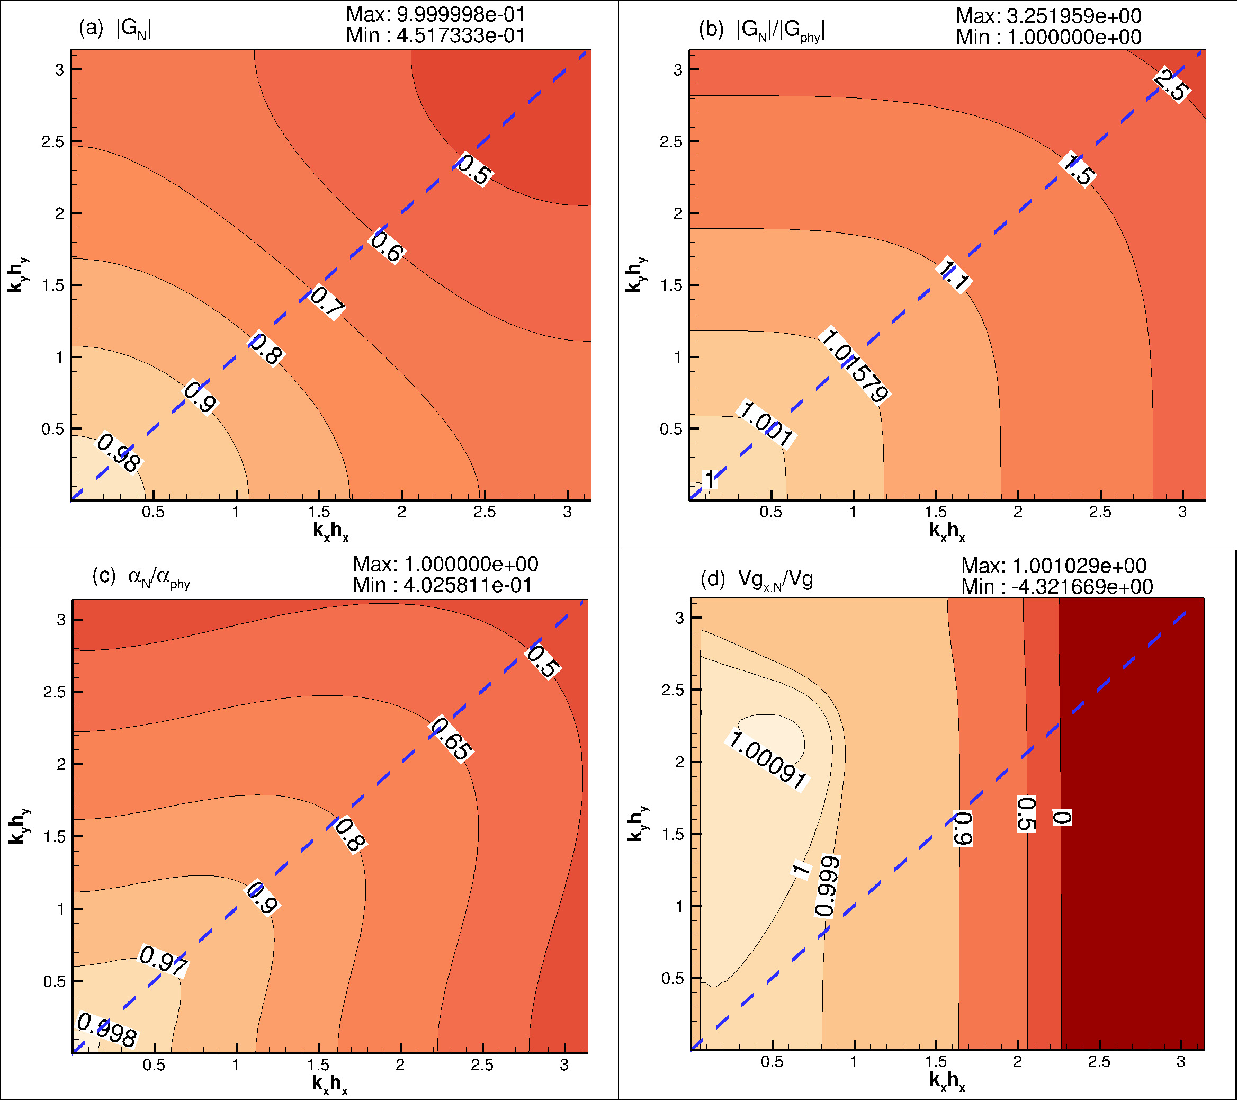
\includegraphics[scale=0.65]{RK4_LELE_CD2_cont.pdf}
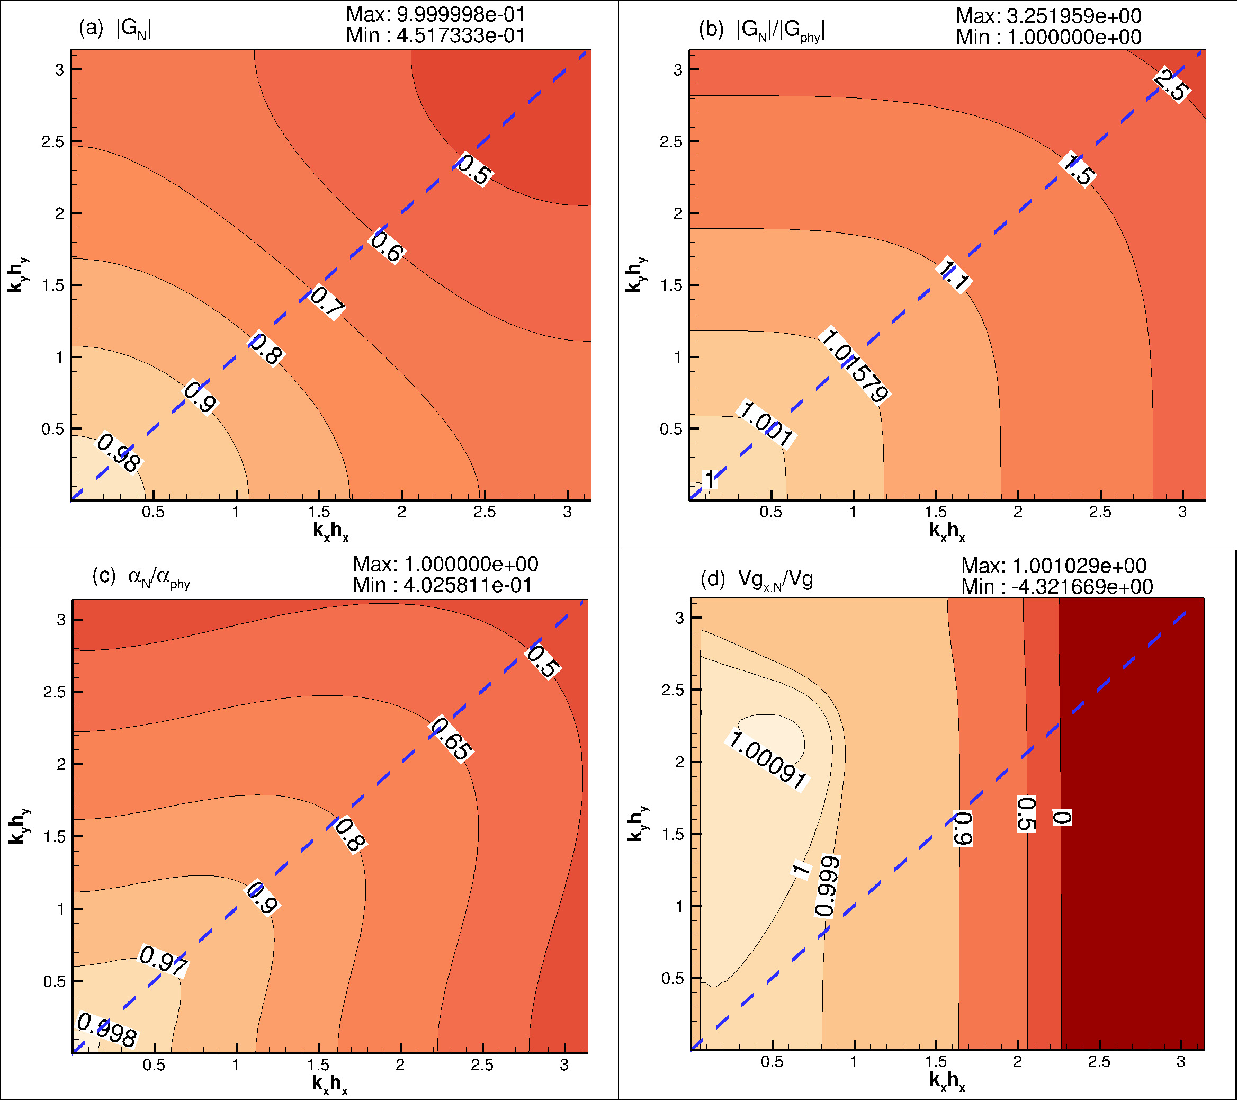
\includegraphics[width=150mm]{RK4_LELE_CD2_cont.pdf}
\end{center}
\raggedleft
\caption{Contour plots of $|G_N|$ (top left), $|G_N|/|G_{phy}|$ (top right), $\alpha_N/\alpha$ (bottom left), $Vg_{xN}/Vg_x$ (bottom right) for RK$_4$-LELE-CD$_2$ scheme at $Nc=0.1$ and $Pe=0.1$.}
\label{fig_lele}
\end{figure}

We adopt four stages Runge-Kutta (RK$_4$) method for time discretization with the sixth order Lele's scheme for discretizing convection term and a second-order central difference (CD$_2$) for the diffusion terms. Evaluated matrices $[C]$ and $[D]$ substituted into Eqn. (20) and then solve Eqn. (19) to find numerical amplification factor ($G_N$) for the scheme and consequently other property ratios such as $|G_N|/|G_{phy}|$, $\alpha_N/\alpha$ and $Vg_{xN}/c_x$ can also be obtained.

\begin{figure}[h]
\begin{center}
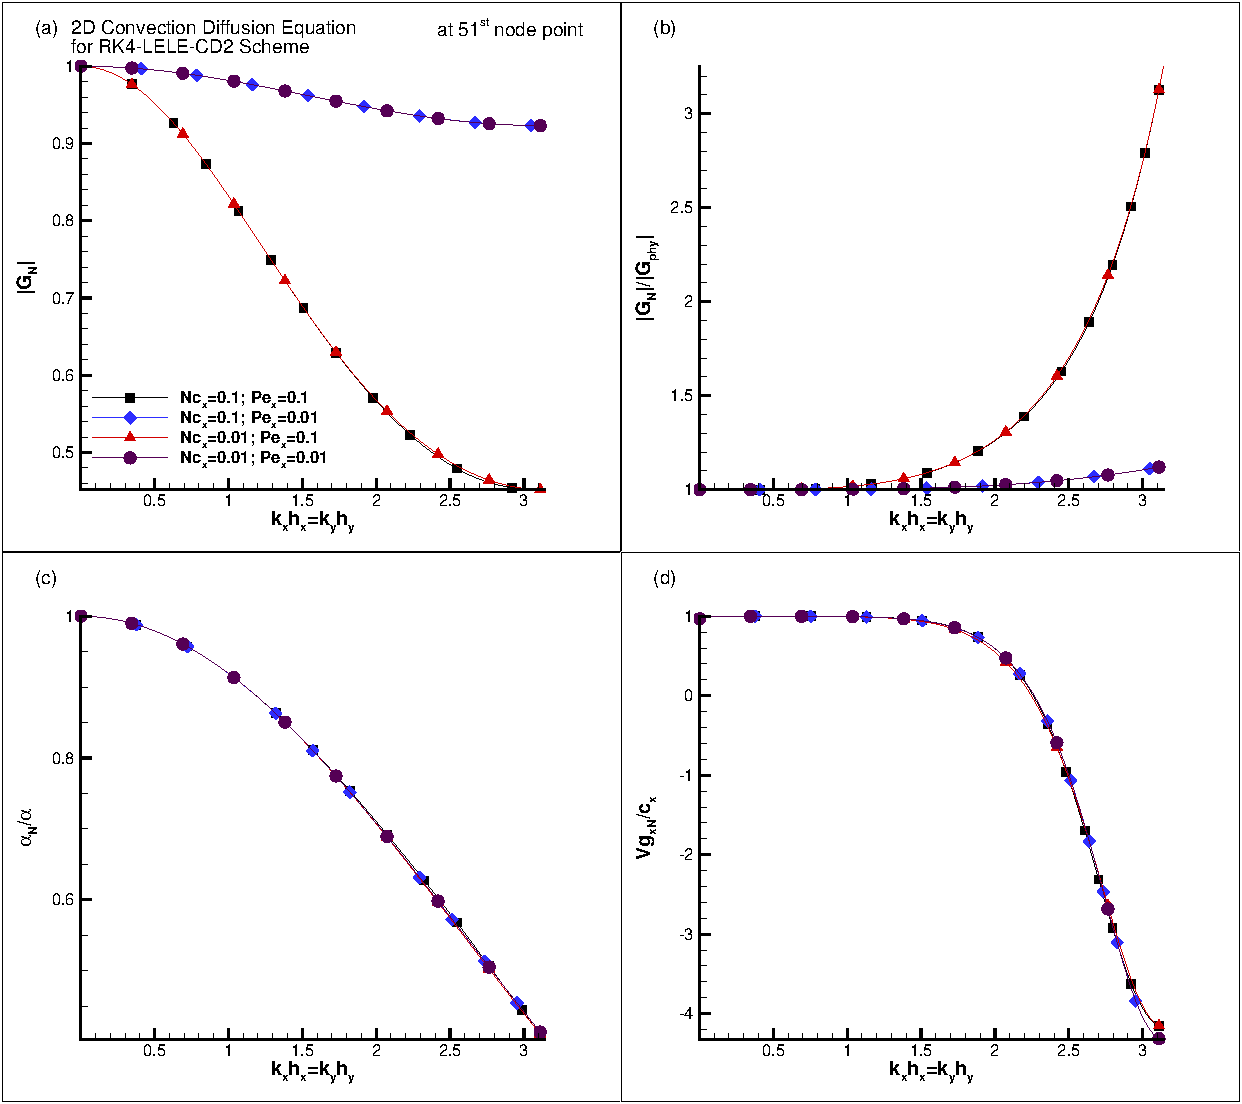
\includegraphics[width=150mm]{prop_LELE_mid_pt.pdf}
\end{center}    
\raggedleft
\caption{Plots of $|G_N|$ (top left), $|G_N|/|G_{phy}|$ (top right), $\alpha_N/\alpha$ (bottom left), $Vg_{xN}/Vg_x$ (bottom right) for RK$_4$-LELE-CD$_2$ scheme for four combination of $Nc$ and $Pe$ written in top left figure at mid or $51^{st}$ node point.}
\label{fig_lele2}
\end{figure}

Fig.\ref{fig_lele} showing contours for four properties of RK$_4$-LELE-CD$_2$ scheme in ($k_xh_x,k_yh_y$)-plane by taking small values of $Nc$ and $Pe$ as 0.1 and 0.1, respectively. Similar contour plots have investigated by taking different combinations of $Nc$, $Pe$, and by considering different wave propagation angle $\theta$ (which we did not show in the paper), found no significant variation even for several numerical schemes. It is evident from Fig. \ref{fig_lele} that the gradient of contours is highest along the diagonal direction of ($k_xh_x,k_yh_y$)-plane (\textit{i.e.} along a straight line from the origin to the Nyquist limit, shown in the figure with blue dashed line) in property diagrams. Therefore it is adequate to plot these properties along a diagonal direction (where $k_xh_x=k_yh_y$), rather than representing contour plots in two-dimensional wavenumber plane, which gives us the liberty to indicate the property curves for multiple combinations of $Nc$ and $Pe$ in the same figure to compare, as shown in Fig.\ref{fig_lele2}.

Fig.\ref{fig_lele2} show the property ratios for four combinations of $Nc$ and $Pe$, indicated with four different line colours and different symbol shapes as shown by the legend in Fig.\ref{fig_lele2}(a). The choice of values for $Nc$ and $Pe$ are based on the same reasoning as concluded in \cite{SUMAN_et_al}, where authors showed that the best accuracy for such compact schemes could be obtained by taking low $Nc$ and $Pe$ values. All the mid-node properties of 2D CDE gets improved by decreasing the value of $Pe$ from 0.1 to 0.01 except $\alpha_N/\alpha$ in Fig.\ref{fig_lele2}(c), which does not show any significant improvement either by reducing $Nc$ or $Pe$. As CD$_2$ is known for its high numerical diffusion, reducing $Pe$ by order of decimal does not affect the overall diffusion of the numerical scheme because matrix $[D]$ dominates the diffusive-error. Decreasing the value of $Nc$ has no significant effect on any property. This scheme shows notably good dispersion property for a wide range of wavenumbers for all four combinations of $Nc$ and $Pe$ taken here, shown in Fig.\ref{fig_lele2}(d).

\subsection{RK$_4$-CD$_2$-CD$_2$ scheme}

Here, we have considered an explicit scheme which is different from previously implimented implicit schemes for convection term. Second order central differencing (CD$_2$) scheme, known to be highly diffusive, for both the spacial derivatives is employed, and the discretized governing equation is given by,
\begin{equation}
\begin{aligned}
\frac{u_{i,j}^{n+1}-u_{i,j}^{n}}{\Delta t}+c_x \frac{u_{i+1,j}^{n}-u_{i-1,j}^{n}}{2\Delta x}+c_y \frac{u_{i,j+1}^{n}-u_{i,j-1}^{n}}{2\Delta y}=&\alpha_x \frac{u_{i+1,j}^{n}-2u_{i,j}^{n}+u_{i-1,j}^{n}}{(\Delta x)^2}\\
+&\alpha_y \frac{u_{i,j+1}^{n}-2u_{i,j}^{n}+u_{i,j-1}^{n}}{(\Delta y)^2}
\end{aligned}
\end{equation}
where, $i$, $j$ denotes the nodal index in $x$- and $y$-directions, respectively, and $n$ the time level. Substituting the spectral representation in the above equation, we obtain the numerical amplification factor written as,
\begin{equation}
(G_N)=1-\frac{N_{cx}}{2}(e^{ikh}-e^{-ikh})-\frac{N_{cy}}{2}(e^{jkh}-e^{-jkh})+Pe_x(e^{ikh}-2+e^{-ikh})+Pe_y(e^{jkh}-2+e^{-jkh})
\end{equation}
where $(G_N)$ is for the node ($i$, $j$) and $N_{cx}$, $N_{cy}$, $Pe_{x}$, $Pe_{y}$ has the usual meaning as before. After this, the numerical properties of this numerical scheme can be easily evaluated from the global spectral analysis as before.

Fig. \ref{fig_CD2} shows a similar trend, as in Fig. \ref{fig_lele2} for $|G_N|$, $|G_N|/|G_{phy}|$, $\alpha_N/\alpha$ and $Vg_{xN}/c_x$ for the same combination of $Nc$ and $Pe$. With comparison to the previous compact scheme, this explicit scheme is easy to implement, but as expected, it shows a highly diffusive nature and, consequently, its effect in numerical group velocity shown in Fig. \ref{fig_CD2}(d). From the figure, it is observed that a component of numerical group velocity lies between values 1 to 0 up to the wavenumbers of $kh=1.5$ and then drops further down to negative values for higher values of wave numbers. Means in a numerical simulation, wavenumbers of a signal (function) higher than $kh=1.5$, will travel in the opposite direction of convection.

\begin{figure}
\begin{center}
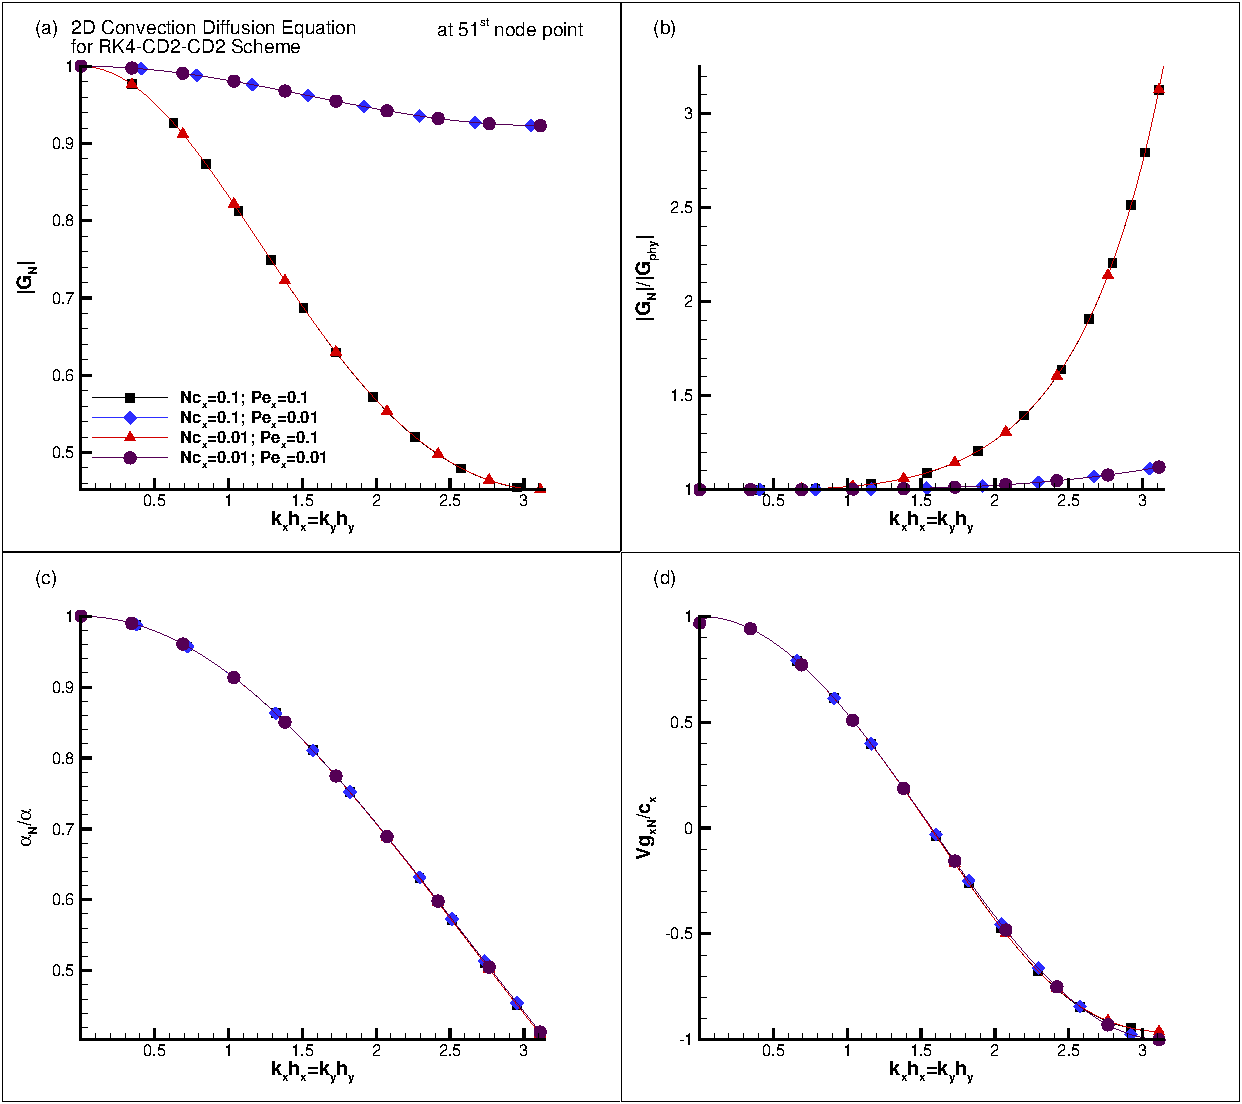
\includegraphics[width=150mm]{prop_CD2_mid_pt.pdf}
\end{center}
\raggedleft
\caption{Plots of $|G_N|$ (top left), $|G_N|/|G_{phy}|$ (top right), $\alpha_N/\alpha$ (bottom left), $Vg_{xN}/Vg_x$ (bottom right) for RK$_4$-CD$_2$-CD$_2$ scheme for four combination of $Nc$ and $Pe$ written in top left figure at mid or $51^{st}$ node point.}
\label{fig_CD2}
\end{figure}

A noteworthy point after implementation of this scheme is that three properties $|G_N|$, $|G_N|/|G_{phy}|$ and $\alpha_N/\alpha$ does not show any appreciable difference in comparison with compact numerical schemes \textit{i.e.} RK$_4$-LELE-CD$_2$ and RK$_4$-OUCS3-CD$_2$ (briefly discussed in \cite{SUMAN_et_al} for implementation in 1D CDE). These three properties are directly related to the numerical diffusion of a numerical scheme. As, we have used second-order central difference CD$_2$ scheme to discretize second-order derivatives in above mentioned numerical schemes; therefore it is evident that high numerical diffusion of CD$_2$ predominates over the high accuracy, high-resolution compact schemes. This encourages one to use different numerical schemes to discretize second-order derivative terms.

%{\subsection{RK$_4$-OUCS3-CD$_2$ scheme}

%{We investigate the impact of employing another compact finite difference for the convection term and four-stage Runge-Kutta method for time integration. Here we consider a second-order, optimized upwind compact scheme (OUCS3), which displays exceptional performance in terms of resolution and accuracy for convection dominated problems [6]. The stencil is given below, and the reader is requested to refer to [7] for further details regarding its design. 

%\begin{equation}
%u_1'=\frac{1}{2h}[-3u_1+4u_2-u_3]
%\end{equation}
%\begin{equation}
%u_2'=\frac{1}{h} \left[ \left( \frac{2\beta}{3}-\frac{1}{3}\right)u_1-\left( \frac{8\beta}{3}+\frac{1}{2}\right)u_2+(4\beta+1)u_3-\left( \frac{8\beta}{3}+\frac{1}{6}\right)u_4+\frac{2\beta}{3}u_5\right]
%\end{equation}
%\begin{equation}
%p_{j-1}u_{j-1}'+u_j'+p_{j+1}u_{j+1}'=\frac{1}{h} \sum_{k=-2}^{2}q_ku_{j+k}
%\end{equation}
%where, $\beta=-0.025\ (\mbox{for }j=2);\ \beta=0.09\ (\mbox{for }j=N-1)$\\
%$p_{j\pm1}=-D\pm\frac{\eta}{60};\ q_{j\pm2}=\pm\frac{F}{4}+\frac{\eta}{300};\ q_{j\pm1}=\pm\frac{E}{2}+\frac{\eta}{30};\ q_{0}=-\frac{11\eta}{150}$\\
%$D=0.3793894912;\ E=1.57557379;\ F=0.183205192;\ \eta=0$\\

%\begin{figure}[h]
%\begin{center}
%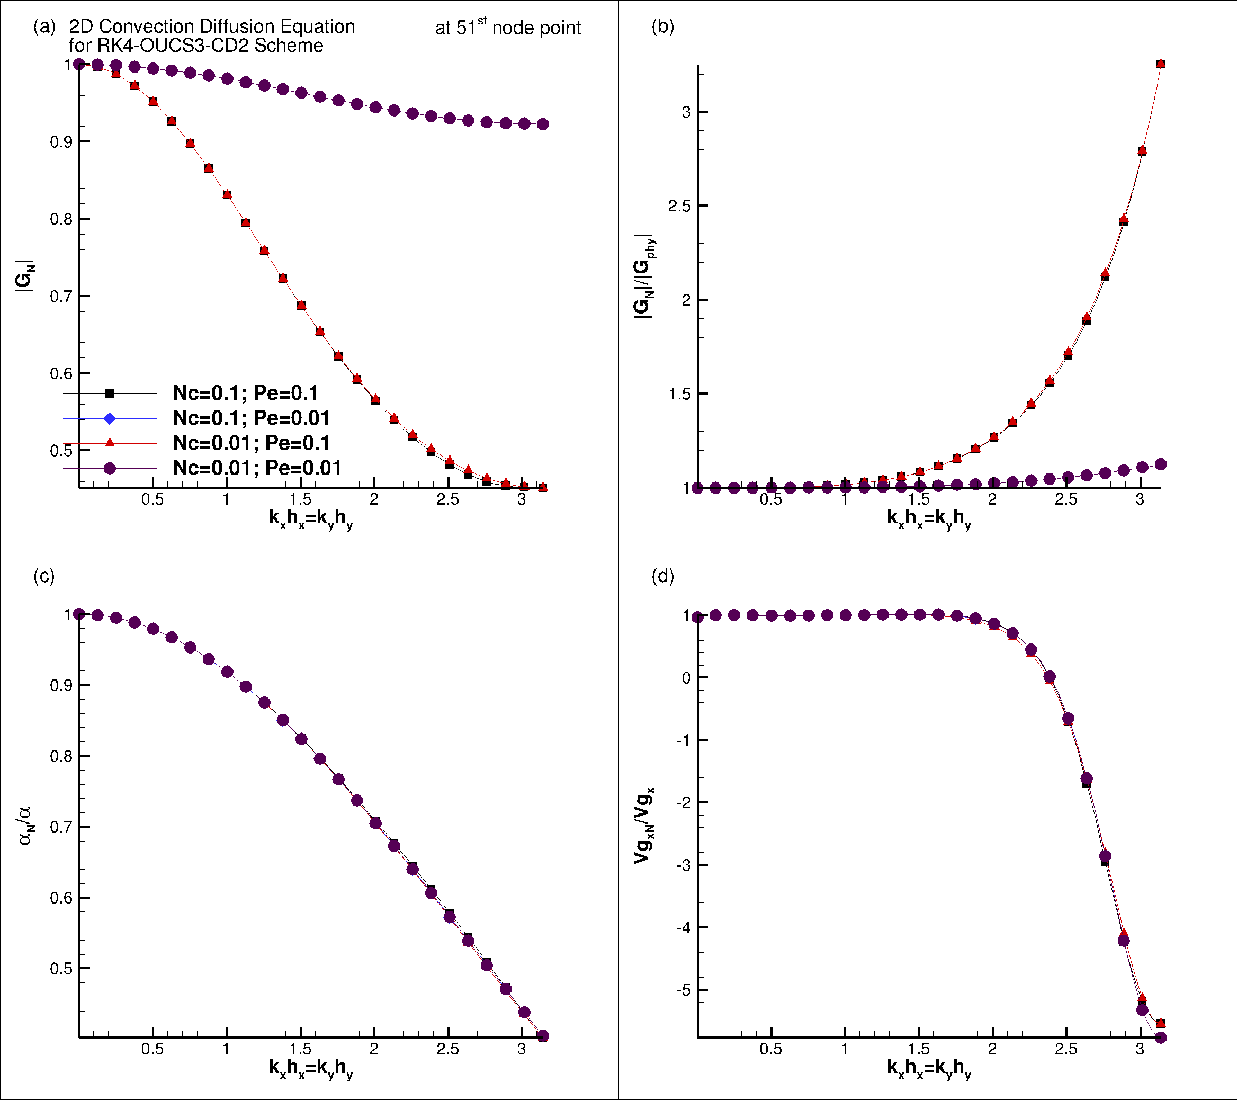
\includegraphics[width=\textwidth]{prop_OUCS3_mid_pt.pdf}
%\end{center}
%\raggedleft
%\caption{RK$_4$-OUCS$3$-CD$_2$ scheme.}
%\label{fig_OUCS3}
%\end{figure}

%{similar boundary closures for the other non-periodic boundary points i.e. for $u_{N-1}'$ and $u_{N}'$ can be considered as used for non-periodic boundary in Eqn (49) and Eqn (50). $A_{mn}$ can be calculated from Eqn. (43), which used to determine the numerical amplification factor by substituting in Eqn. (42). Then ratios $\frac{|G_N|}{G_{phy}}$, $\frac{\alpha_N}{alpha}$, and $\frac{(V_{gx})_N}{V_{gx}}$ can be calculated for this numerical method, as before.

%{We investigate the performance of the scheme at the interior node for non-periodic boundary conditions of the two-dimensional computational domain. Fig.\ref{fig_OUCS3} shows the properties for the same combination of $Nc$ and $Pe$ values. The scheme's superior accuracy can be immediately noted form the plots. For $Pe=0.01$, the numerical amplification remains closer to the physical amplification for a broader range of wavenumbers, as noted from Fig.\ref{fig_OUCS3}(b). The mid node properties for this scheme are very close to the previous numerical scheme, but in terms of numerical group velocity, this scheme shows the more negative value at high wavenumbers close to the Nyquist limit. This scheme also shows the significant overall improvement of properties by reducing values of $Pe$.}

\subsection{RK$_4$-LELE-LELE$^2$ scheme}

Here we investigate the impact of compact finite difference scheme employed for the convection as well as for diffusion term of CDE and four-stage Runge-Kutta method for time integration. We consider two distinct sixth-order Lele's compact schemes deduced for first and second-order derivatives, which displays exceptional performance in terms of resolution and accuracy for a convection-diffusion problem. The stencils are given below, and the reader is requested to refer to \cite{LELE1992} for further details regarding its design.

\begin{figure}
\begin{center}
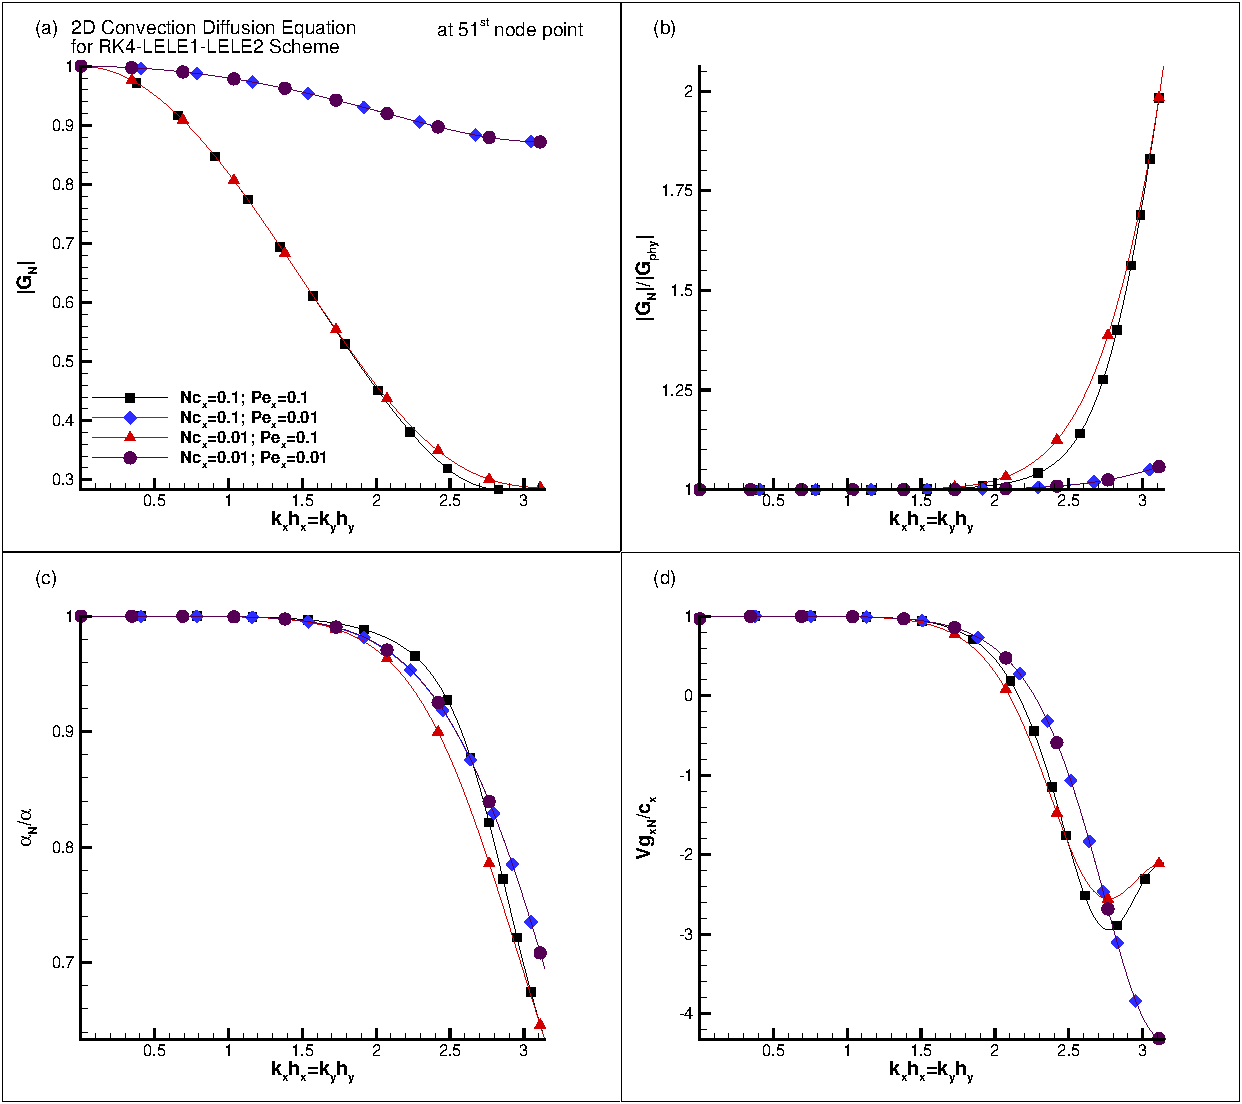
\includegraphics[width=150mm]{prop_RK4_LELE_LELE.pdf}
\end{center}
\raggedleft
\caption{Plots of $|G_N|$ (top left), $|G_N|/|G_{phy}|$ (top right), $\alpha_N/\alpha$ (bottom left), $Vg_{xN}/Vg_x$ (bottom right) for RK$_4$-Lele-Lele$_2$ scheme for four combination of $Nc$ and $Pe$ written in top left figure at mid or $51^{st}$ node point.}
\label{fig_LELE_2}
\end{figure}

By applying the general principle of compact differencing, to evaluate derivatives of Lele's scheme from the following stencils
\begin{equation}
\alpha_1 u_{j-1}'+u_j'+\alpha_1 u_{j+1}'=\frac{a_1}{2h} (u_{j+1}-u_{j-1})+\frac{b_1}{4h} (u_{j+2}-u_{j-2})
\end{equation}
Eqn. (28) is a sixth order accurate scheme obtained for the evaluation of first derivative, with $\alpha_1=1/3$, $a_1=14/9$ and $b_1=1/9$. 
\begin{equation}
\alpha_2 u_{j-1}''+u_j''+\alpha_2 u_{j+1}''=\frac{a_2}{h^2} (u_{j+1}-2u_{j}+u_{j-1})+\frac{b_2}{4h^2} (u_{j+2}-2u_{j}+u_{j-2})
\end{equation}
Eqn. (29) is also formally a sixth order accurate scheme obtained for the evaluation of second derivative, with $\alpha_2=2/11$, $a_2=12/11$ and $b_2=3/11$.
For non-periodic boundaries following explicit boundary closure are applied:
\begin{equation}
u_1'=\frac{1}{2h}(-2u_1+2u_2)
\end{equation}
\begin{equation}
u_1''=\frac{1}{h^2}[u_1-2u_2+u_3]
\end{equation}
\begin{equation}
u_2'=\frac{1}{2h}(-u_1+u_3)
\end{equation}
\begin{equation}
u_2''=\frac{1}{h^2}[u_1-2u_2+u_3]
\end{equation}

From Fig. \ref{fig_LELE_2} it is evident that this scheme implies a significant overall improvement of properties for small values of $Nc$ and $Pe$.

\subsection{RK$_4$-NCCD scheme}
In this section we investigate another popular variant of compact difference schemes called the combined compact difference (CCD) scheme for spatial discretization, and are specially used to simultaneously evaluate both first and second order derivatives \cite{CHU_AND_FAN, ZHOU_ET_AL}. In this paper we have considered the improved CCD scheme (NCCD) from \cite{SENGUPTA_Et_al_4} for the present analysis and the stencil is given below. The reader is requested to consult above references for further details. Mid-node stencils are given by,
\begin{equation}
\frac{7}{16}(u_{j+1}'+u_{j-1}')+u_j'-\frac{h}{16}(u_{j+1}''-u_{j-1}'')=\frac{15}{16h}(u_{j+1}-u_{j-1}),
\end{equation}
\begin{equation}
\frac{9}{8h}(u_{j+1}'-u_{j-1}')+u_j''-\frac{1}{8}(u_{j+1}''-u_{j-1}'')=\frac{3}{h^2}(u_{j+1}-2u_j+u_{j-1}),
\end{equation}

and boundary node stencils are given by,
\begin{equation}
u_1'=\frac{1}{2h}[-3u_1+4u_2-u_3]
\end{equation}
\begin{equation}
u_1''=\frac{1}{h^2}[u_1-2u_2+u_3]
\end{equation}
\begin{equation}
u_2'=\frac{1}{h} \left[ \left( \frac{2\beta}{3}-\frac{1}{3}\right)u_1-\left( \frac{8\beta}{3}+\frac{1}{2}\right)u_2+(4\beta+1)u_3-\left( \frac{8\beta}{3}+\frac{1}{6}\right)u_4+\frac{2\beta}{3}u_5\right]
\end{equation}
\begin{equation}
u_2''=\frac{1}{h^2}[u_1-2u_2+u_3]
\end{equation}
\begin{equation}
\begin{aligned}
u_{N-1}'=-\frac{1}{h} \left[ \left( \frac{2\beta}{3}-\frac{1}{3}\right)u_N-\left( \frac{8\beta}{3}+\frac{1}{2}\right)u_{N-1}+(4\beta+1)u_{N-2}
-\left( \frac{8\beta}{3}+\frac{1}{6}\right)u_{N-3}+\frac{2\beta}{3}u_{N-4}\right]
\end{aligned}
\end{equation}

\begin{figure}[h]
\begin{center}
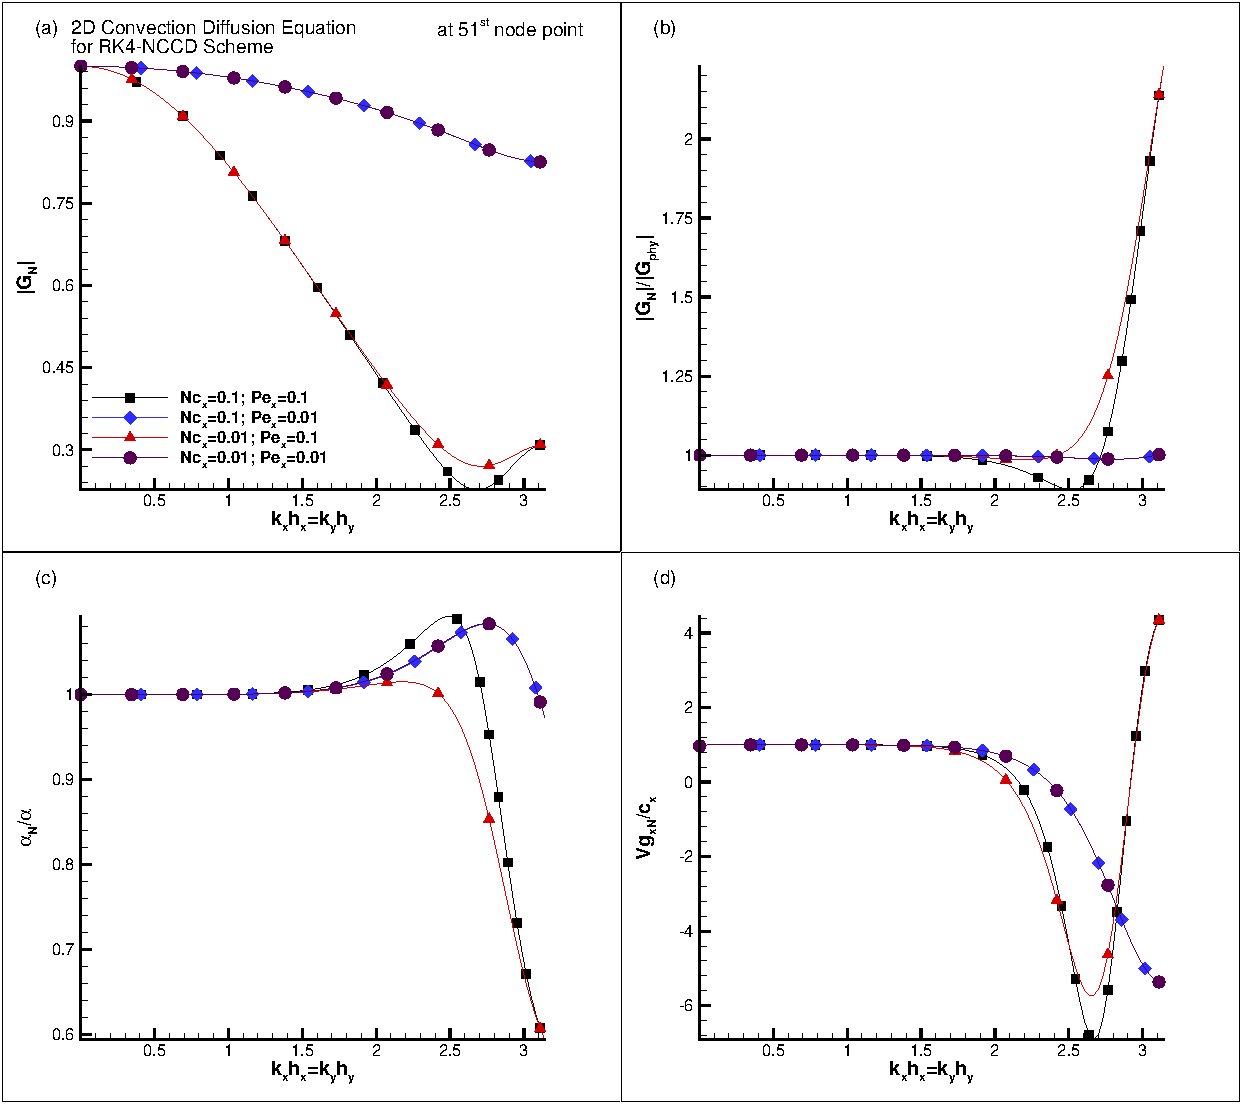
\includegraphics[width=150mm]{prop_NCCD_mid_pt.pdf}
\end{center}
\raggedleft
\caption{Plots of $|G_N|$ (top left), $|G_N|/|G_{phy}|$ (top right), $\alpha_N/\alpha$ (bottom left), $Vg_{xN}/Vg_x$ (bottom right) for RK$_4$-NCCD-CD$_2$ scheme for four combination of $Nc$ and $Pe$ written in top left figure at mid or $51^{st}$ node point.}
\label{fig_NCCD}
\end{figure}

\begin{equation}
u_{N-1}''=\frac{1}{h^2}[u_N-2u_{N-1}+u_{N-2}]
\end{equation}
\begin{equation}
u_{N}'=\frac{1}{2h}[3u_N-4u_{N-1}+u_{N-2}]
\end{equation}
\begin{equation}
u_{N}''=\frac{1}{h^2}[u_N-2u_{N-1}+u_{N-2}]
\end{equation}
where, $\beta=-0.025\ (\mbox{for }j=2);\ \beta=0.09\ (\mbox{for }j=N-1)$,\\
here primes indicate derivatives, as before. The solution of these simultaneous equations can be expressed as, 
\begin{equation}
\begin{aligned}
\{u'\}&=\frac{1}{h}[C]\{u\}\\
\{u''\}&=\frac{1}{h^2}[D]\{u\}
\end{aligned}
\end{equation}

where matrices $[C]$ and $[D]$ are presented in [18]. Block tridiagonal matrix algorithm (TDMA) is employed to calculate the inverses to obtain $[C]$ and $[D]$. After this step, the same approach described for the compact scheme adopted to calculate the numerical amplification factor and hence the other properties at mid-node of the computational domain.

Fig.\ref{fig_NCCD} shows the error properties for different values of $Nc$ and $Pe$. The sixth order accurate combined compact scheme (NCCD) shows a considerable improvement in all four ratios by reducing the values of $Pe$ for a broader range of wavenumbers, especially the numerical amplification factor, as shown in Fig.\ref{fig_NCCD}(b). Enhancement in the numerical diffusion shown in Fig.\ref{fig_NCCD}(c), which remains very close to its physical values for a much broader range of wavenumbers by taking $Pe=0.01$.


\section{Non-Periodic Boundary closure}

Application with non-periodic boundaries are widespread, which involves wall-bounded computational domains. For problems with periodic boundary conditions, matrices $[A_1]$, $[B_1]$, $[A_2]$ and $[B_2]$, in Eqn. (24) and Eqn. (25), are periodic symmetric matrices. However, for many practical problems periodic boundary conditions are not applicable and one-sided stencils needed near boundaries, as considered in the last section to calculate global spectral analysis at mid-nodes, making matrices $[A_1]$, $[B_1]$, $[A_2]$ and $[B_2]$ non-symmetric.

\begin{figure}[h]
\begin{center}
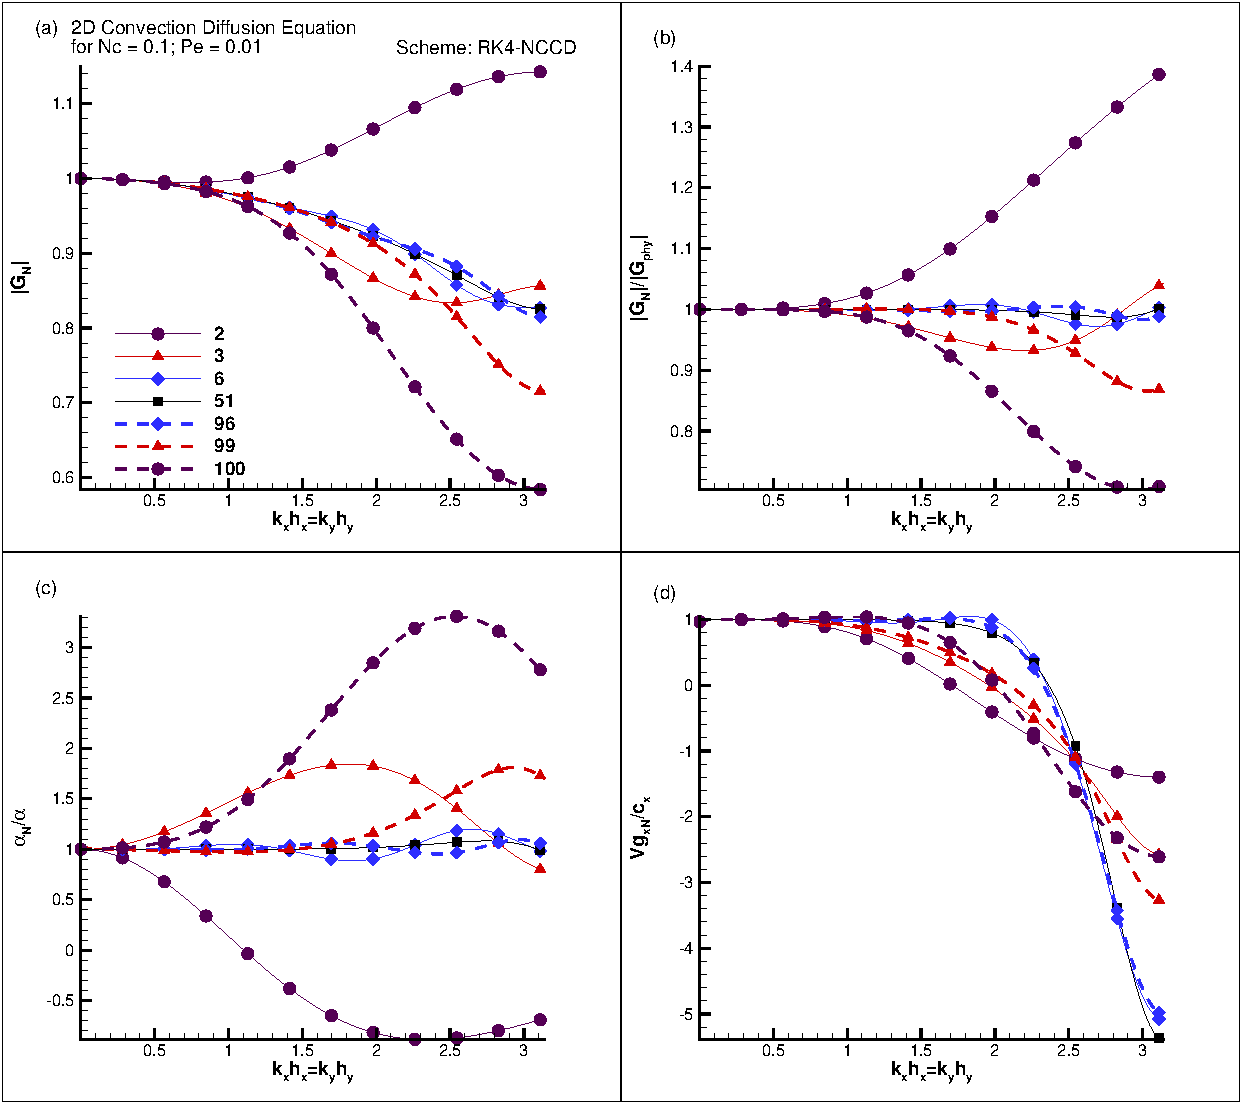
\includegraphics[width=150mm]{prop_NCCD_nodes.pdf}
\end{center}
\raggedleft
\caption{Plots of $|G_N|$ (top left), $|G_N|/|G_{phy}|$ (top right), $\alpha_N/\alpha$ (bottom left), $Vg_{xN}/Vg_x$ (bottom right) for RK$_4$-NCCD-CD$_2$ scheme at different nodes/points, indicated in top left figure, for $Nc=0.1$ and $Pe=0.01$.}
\label{fig_NCCD_nodes}
\end{figure}

In this section, we will present the properties of 2D CDE for adjacent to the boundary nodes; the properties for near boundary nodes display very different behavior and accuracy than mid-node. Properties for near boundary nodes are non-identical and shows significant variation in wavenumber plane for different numerical schemes, and their variation with $Nc$ and $Pe$ are also distinct.

Fig.\ref{fig_NCCD_nodes} represent near boundaries spectral properties for the NCCD scheme, which supposed to have better error properties, among others, as discussed in the previous section. The comparison between all schemes for mid-node properties is presented and discussed in the results section. Here Peclet number $Pe=0.01$ has been adopted with $Nc=0.1$ to calculated property ratios for seven distinct boundary nodes. Three near boundary nodes corresponding either side of the non-periodic boundary, total six nodes, and a mid-node is also included to compare curves. In Fig.\ref{fig_NCCD_nodes} curves for nod-2 and node-100 are the corresponding nodes; hence, their line color in the plot is the same, similarly for other near boundary corresponding nodes. From Fig.\ref{fig_NCCD_nodes}(c), all near boundary nodes, including mid-node, shows numerical diffusion either close to or greater than physical diffusion for a wide range of wavenumbers except for node-2. Hence the ratio $|G_N|/|G_{phy}|$ for these nodes in Fig.\ref{fig_NCCD_nodes}(b) shows numerical amplification factor either close to or less than the physical amplification factor for most of the wavenumbers. For node-2, the figure shows a large part of numerical diffusion in the negative side of $\alpha_N/\alpha$ plot, and its effect reflected in $|G_N|$ plot in Fig.\ref{fig_NCCD_nodes}(a) the curve reaches to more than unit value. The phenomena related to such behavior of properties will be explained in the next section called \textit{focusing}.

Dispersion property in Fig.\ref{fig_NCCD_nodes}(d) for near boundary nodes shows less accuracy for a wide range of wave numbers similar to the other three properties. It is worth to note that wavenumber components with negative group velocity exhibit the presence of q-waves or upstream propagating waves as described in \cite{SUMAN_et_al}.

The analysis shows that the local error due to inherent approximation included in the formulation of boundary closures. It is also inevitable that this boundary formulation maintains global conservation; therefore, their effects percolate consequently affect the interior nodes. GSA helps to quantify the errors due to boundary treatment, as typically the global error many times dominated by the boundary error.

\section{Error Dynamics for Convection-Diffusion Equation}

Here we demonstrate the error dynamics for the convection-diffusion equation. For the analysis of space-time discretization schemes, the linear convection-diffusion acquire as a model that represents a linear form of Navier-Stokes equation (NSE) used for practical flow problems, written as
\begin{equation}
\frac{\partial u}{\partial t}+c\frac{\partial u}{\partial x}=\alpha \frac{\partial^2 u}{\partial x^2}
\end{equation}
As a mathematical equation, Eqn. (45) represents convection of an initial condition to the right with a constant rate of diffusion, at a phase speed of $c$, and the diffusivity/rate of diffusion as $\alpha$ all times. Hence this equation gives a basis for testing numerical methods for the solution of NSE with accuracy by obeying correct error propagation, i.e., alleviation in properties like dispersion, diffusion, and dissipation error, as in \cite{SENGUPTA_et_al_2, SENGUPTA_et_al_3}.

We represent the unknown by its Fourier transform at the $j$th node of a uniformly spaced discrete grid of spacing $h$ as, $u(x_j,t)=\int \hat{U}(k,t)e^{ikx_j}dk$ and the exact spatial first and second derivatives at the same node is given by, $[u_j']_{exact}=\int ik\hat{U}e^{ikx_j}dk$ and $[u_j'']_{exact}=-\int k^2\hat{U}e^{ikx_j}dk$. While solving Eqn. (45) by discrete methods, the spatial derivatives $u_j'$ and $u_j''$ (denoted by prime/s) can be written equivalently as,
\begin{equation}
\begin{aligned}
[u_j']_{numerical}&=\int ik_{eq}^{(1)}\hat{U}(k,t)e^{ikx_j}dk \\
[u_j'']_{numerical}&=\int k_{eq}^{(2)}\hat{U}(k,t)e^{ikx_j}dk
\end{aligned}
\end{equation}

Numerically in a finite-domain the same derivatives are estimated as, $\{u'\}=\frac{1}{h}[C]\{u\}$ and $\{u''\}=\frac{1}{h^2}[D]\{u\}$. One can obtain an appropriate matrices $[C]$ and $[D]$ for finite-domain periodic or non-periodic problems, with the dimension of matrices corresponding to the number of nodes. However using above relations, one can relate the function at $j$th and $l$th node by 
\begin{equation}
\int \hat{U}(k,t)e^{ikx_l}dk=\int \hat{U}(k,t)e^{ik(x_l-x_j)}e^{ikx_j}dk
\end{equation}
one can therefore represent the first derivative at the $j$th node by the variable at the same node from the following equation
\begin{equation}
u_j'=\int \frac{1}{h} \sum_{i=1}^{N} C_{jl}\hat{U}(k,t) e^{ik(x_l-x_j)}e^{ikx_j}dk
\end{equation}
where $C_{jl}$ are the entries of the $[C]$ matrix. Comparing Eqn. (46) with Eqn. (48), we note that 
\begin{equation}
[ik_{eq}^{(1)}]_j=\frac{1}{h} \sum C_{jl}e^{ik(x_l-x_j)}
\end{equation}
similarly by evaluating for second derivative,
\begin{equation}
-[k_{eq}^{(2)}]_j=\frac{1}{h^2} \sum D_{jl}e^{ik(x_l-x_j)}
\end{equation}

Although in physical plane computations, $C_{jl}$ and $D_{jl}$ are real, in general $k_{eq}^{(1)}$ and $k_{eq}^{(2)}$ are complex numbers as, 
\begin{equation}
i\int k_{eq}^{(1)}\hat{U}(k,t)e^{ikx_j}dk= i\int k_{eq}^{(1)}|_{real}\hat{U}(k,t)e^{ikx_j}-\int k_{eq}^{(1)}|_{imag}\hat{U}(k,t)e^{ikx_j}
\end{equation}
real part of $k_{eq}^{(1)}$ indicating spectral resolution of the scheme and the imaginary part of $k_{eq}^{(1)}$ indicating added numerical diffusion.

Similarly, the real part of $k_{eq}^{(2)}$ represents scale-wise dissipation, and the imaginary part represents added numerical dispersion for a numerical method by determining the entries of the matrices $[C]$ and $[D]$.

Other important numerical properties are obtained via the spectral representation in Eqn. (45), that gives
\begin{equation}
\int \left[ \frac{d \hat{U}}{d t} + \frac{c}{h}\sum \hat{U}C_{jl}e^{ik(x_l-x_j)} - \frac{\alpha}{h^2}\sum \hat{U}D_{jl}e^{ik(x_l-x_j)} \right]e^{ikx_j}dk=0
\end{equation}

Since the above equation is true for all wavenumbers, the integrand must be zero for any $k$. The implicit condition of Eqn. (52), can be reinterpreted as,
\begin{equation}
\frac{d\hat{U}}{\hat{U}}=-\left[\frac{c\Delta t}{h}\right] \sum_{l=1}^N C_{jl}e^{ik(x_l-x_j)} + \left[\frac{\alpha \Delta t}{h^2}\right] \sum_{l=1}^N D_{jl}e^{ik(x_l-x_j)}
\end{equation}

We note that two factors in squared bracket on the right-hand side are nothing but the CFL number ($Nc$) and Peclet number ($Pe$), respectively. Since the right-hand side of Eqn. (53) is node-dependent, we can express the left hand side in terms of the nodal numerical amplification factor ($G_j$), therefore
\begin{equation}
G_j=G(x=x_j)=1-Nc \sum_{l=1}^N C_{jl}e^{ik(x_l-x_j)} + Pe \sum_{l=1}^N D_{jl}e^{ik(x_l-x_j)}
\end{equation}
for the Euler time discretization scheme. Similarly, one can obtain $G_j$ for other time discretization schemes and for the four-stage Runge-Kutta time integration scheme, this has been obtained in \cite{sengupta2013high} and \cite{SENGUPTA_et_al_2, SENGUPTA_et_al_7} as,
\begin{equation}
G_j=1-A_j+\frac{A_j^2}{2}-\frac{A_j^3}{6}+\frac{A_j^4}{24}
\end{equation}
where $A_j=Nc\sum C_{jl}e^{ik(x_l-x_j)}-Pe\sum D_{jl}e^{ik(x_l-x_j)}$. A similar relation for general class of the Runge-Kutta methods is given in \cite{BHAUMIK2013}. The present relation is for the fourth order Runge-Kutta scheme obtained for any nodes of non-periodic problem. Such full-domain analysis for some explicit and implicit numerical discretization schemes are available in \cite{sengupta2013high}. While the amplification factor can be a source of error, additional errors can arise due to numerical diffusion, dispersion and dissipation, as described in the previous section. If we represent the initial condition for Eqn. (45) as given by
\begin{equation}
u(x_j,t=0)=u_j^0=\int A_0(k)e^{ikx_j}dk
\end{equation}
then the general numerical solution of Eqn. (45) at any arbitrary time can be obtained as,
\begin{equation}
u_j^n=\int A_0(k)e^{-\alpha_Nk^2t}e^{ik(x_j-c_Nt)}dk
\end{equation}
Thus the phase of the solution is determined by $n\beta_j=kc_Nt$, where $c_N$ is the numerical phase speed. The coefficient $\alpha_N$ in exponent of Eqn. (57) is to evaluate change in the magnitude of initial condition and to incorporate numerical amplification and diffusion in the magnitude of initial condition, $\alpha_N$ called numerical diffusivity or numerical coefficient of diffusion. Although the physical speed and coefficient of diffusion are constant for all wavenumbers, this analysis shows that the numerical phase speed and diffusion coefficient are wavenumber dependent \textit{i.e.} the numerical solution is diffusive as well as dispersive in nature, in contrast with the physical dispersion relation. The implication of this simple difference can be very important, as demonstrated below.

The general numerical solution of Eqn. (45) is denoted as,
\begin{equation}
u_N=\int A_0e^{-\alpha_Nk^2t}e^{ik(x-c_Nt)}dk
\end{equation}

The fact that $c_N \neq c$, $\alpha_N\neq \alpha$, and they are a function of $k$ has been used to explain the shortcomings of some multi-time step integration methods in \cite{sengupta2004}. Since the numerical dispersion relation is given as $\omega_N=kc_N-i\alpha_Nk^2$, instead of $\omega=kc-i\alpha k^2$. Based on these relations, numerical phase speed, group velocity, and diffusion coefficient have already derived in the previous section.

The characteristics of some well known numerical methods have already reported in \cite{SENGUPTA_et_al_2, SENGUPTA_et_al_3, SENGUPTA_et_al_7} in terms of the amplification rate, numerical phase speed, group velocity, and diffusion coefficient. The primary purpose of the present work is to show the consequence of such dispersion, with diffusion to explain error growth for Eqn. (45) and thereby draw general observations for error dynamics of linear systems, as shown next.

If we define the computation error as $e(x,t)=u(x,t)-u_N$, then we can obtain the governing equation for its dynamics in the following manner. Using Eqn. (58) one obtains
\begin{equation}
\frac{\partial u_N}{\partial x}=\int ikA_0 e^{-\alpha_Nk^2t}e^{ik(x-c_Nt)}dk
\end{equation}
\begin{equation}
\frac{\partial^2 u_N}{\partial x^2}=-\int k^2A_0 e^{-\alpha_Nk^2t}e^{ik(x-c_Nt)}dk
\end{equation}
and
\begin{equation}
\frac{\partial u_N}{\partial t}=-\int (\alpha_Nk^2+ikc_N) A_0 e^{-\alpha_Nk^2t}e^{ik(x-c_Nt)}dk \
\end{equation}
Thus, the error propagation equation is given by
\begin{equation}
\frac{\partial e}{\partial t}+c\frac{\partial e}{\partial x}-\alpha\frac{\partial^2 e}{\partial x^2}=-\frac{\partial u_N}{\partial t}-c\frac{\partial u_N}{\partial x}+\alpha\frac{\partial^2 u_N}{\partial x^2}
\end{equation}
substituting from Eqns. (59), (60) and (61)
\begin{equation}
\begin{aligned}
\frac{\partial e}{\partial t}+c\frac{\partial e}{\partial x}-\alpha\frac{\partial^2 e}{\partial x^2}&=\int ikc_NA_0 e^{-\alpha_Nk^2t}e^{ik(x-c_Nt)}dk - c\int ikA_0 e^{-\alpha_Nk^2t}e^{ik(x-c_Nt)}dk\\ &+ \int \alpha_N k^2A_0 e^{-\alpha_Nk^2t}e^{ik(x-c_Nt)}dk - \alpha \int k^2A_0 e^{-\alpha_Nk^2t}e^{ik(x-c_Nt)}dk
\end{aligned}
\end{equation}
first and third term in the right hand side can be simplified to
\begin{equation}
\begin{aligned}
\int ikc_NA_0 e^{-\alpha_Nk^2t}e^{ik(x-c_Nt)}dk &=c_N \int ikA_0 e^{-\alpha_Nk^2t}e^{ik(x-c_Nt)}dk\\ &- \int \frac{dc_N}{dk} \left[\int ikA_0 e^{-\alpha_Nk^2t}e^{ik(x-c_Nt)}dk \right] dk
\end{aligned}
\end{equation}
\begin{equation}
\begin{aligned}
\int \alpha_N k^2A_0 e^{-\alpha_Nk^2t}e^{ik(x-c_Nt)}dk &=\alpha_N \int k^2A_0 e^{-\alpha_Nk^2t}e^{ik(x-c_Nt)}dk\\ &- \int \frac{d\alpha_N}{dk} \left[\int k^2A_0 e^{-\alpha_Nk^2t}e^{ik(x-c_Nt)}dk \right] dk
\end{aligned}
\end{equation}
substituting into the Eqn. (63)
\begin{equation}
\begin{aligned}
\frac{\partial e}{\partial t}+c\frac{\partial e}{\partial x}-\alpha\frac{\partial^2 e}{\partial x^2}&=(c_N-c)\int ikA_0 e^{-\alpha_Nk^2t}e^{ik(x-c_Nt)}dk\\ &+ (\alpha-\alpha_N)\int k^2A_0 e^{-\alpha_Nk^2t}e^{ik(x-c_Nt)}dk\\ & - \int \frac{dc_N}{dk} \left[\int ikA_0 e^{-\alpha_Nk^2t}e^{ik(x-c_Nt)}dk \right]dk\\ & + \int \frac{d\alpha_N}{dk} \left[\int k^2A_0 e^{-\alpha_Nk^2t}e^{ik(x-c_Nt)}dk\right] dk\\
\end{aligned}
\end{equation}
by simplifying this equation, we will get,
\begin{equation}
\begin{aligned}
\frac{\partial e}{\partial t}+c\frac{\partial e}{\partial x}-\alpha\frac{\partial^2 e}{\partial x^2}=&-c\left(1-\frac{c_N}{c}\right)\frac{\partial u_N}{\partial x}+ \alpha\left(1-\frac{\alpha_N}{\alpha}\right)\frac{\partial^2 u_N}{\partial x^2}\\ & - \int \frac{dc_N}{d(kh)} \left( \frac{\partial u_N}{\partial x} \right) d(kh)+ \int \frac{d\alpha_N}{d(kh)} \left( \frac{\partial^2 u_N}{\partial x^2} \right) d(kh)
\end{aligned}
\end{equation}
by substituting $\frac{dc_N}{dk}=\frac{Vg_N-c_N}{k}$, this equation can also be written as;
\begin{equation}
\begin{aligned}
\frac{\partial e}{\partial t}+c\frac{\partial e}{\partial x}-\alpha\frac{\partial^2 e}{\partial x^2}=&-c\left[1-\frac{c_N}{c}\right]\frac{\partial u_N}{\partial x}+ \alpha\left[1-\frac{\alpha_N}{\alpha}\right]\frac{\partial^2 u_N}{\partial x^2}\\ & - c \int \left[\frac{Vg_N-c_N}{c(kh)}\right] \left( \frac{\partial u_N}{\partial x} \right) d(kh)+ \alpha \int \left[ \frac{d(\alpha_N/\alpha)}{d(kh)}\right] \left( \frac{\partial^2 u_N}{\partial x^2} \right) d(kh)
\end{aligned}
\end{equation}

This error propagation equation is comprehensive, contrary to that obtained by several authors in the past using the assumption made in von Neumann analysis, where the right-hand side identically has taken to be zero on the premise that $c_N\equiv c$, $\alpha_N\equiv \alpha$, \textit{i.e.} there are no numerical diffusion and dispersion errors and the numerical method is entirely neutral. Some combinations of numerical parameters ($\textit{e.g.}$ Peclet number or $Pe$ and Courant-Friedrichs-Lewy (CFL) number \cite{NEUMANN_at_al} or $Nc$ in the present study) for solving analysis lead to numerical instability, with an error growing faster than predicted by von Neumann error analysis \cite{SENGUPTA_et_al_2}. In \cite{Vichnevetsky_et_al}, this has studied by solving the convection equation using finite difference and finite element methods. A mismatch between error estimate by von Neumann analysis and numerical solution attributed to diffusion and dispersion of numerical methods. Noting from the first term in the right-hand side of Eqn. (68) that the dispersion error to dramatically increase when the numerical solution displays sharp spatial variation. The second term in the right-hand of Eqn. (68) suggest that the diffusion errors increases when there is a significant change in the second derivatives. In \cite{KREISS1972, Swartz1974, Trefethen_et_al}, phase error ($c-c_N$) reported for monochromatic waves for periodic problems. Its influence on signal error not reported, but it speculated that the phase error could be reduced by grid refinement while keeping $Nc$ the same. A similar presumption also attributes to give an opinion that refining the computation grid can also reduce the dispersion errors, due to numerical diffusion, while keeping $Pe$ same. Nevertheless, the study of error propagation equation suggests that these errors can be controlled by careful analysis of numerical schemes based on GSA and analysis of error matrices shown in Eqn. (68). The third and fourth term in the right-hand side of Eqn. (68) shows the errors related to numerical dispersion and dissipation, respectively.

\begin{figure}[h]
\begin{center}
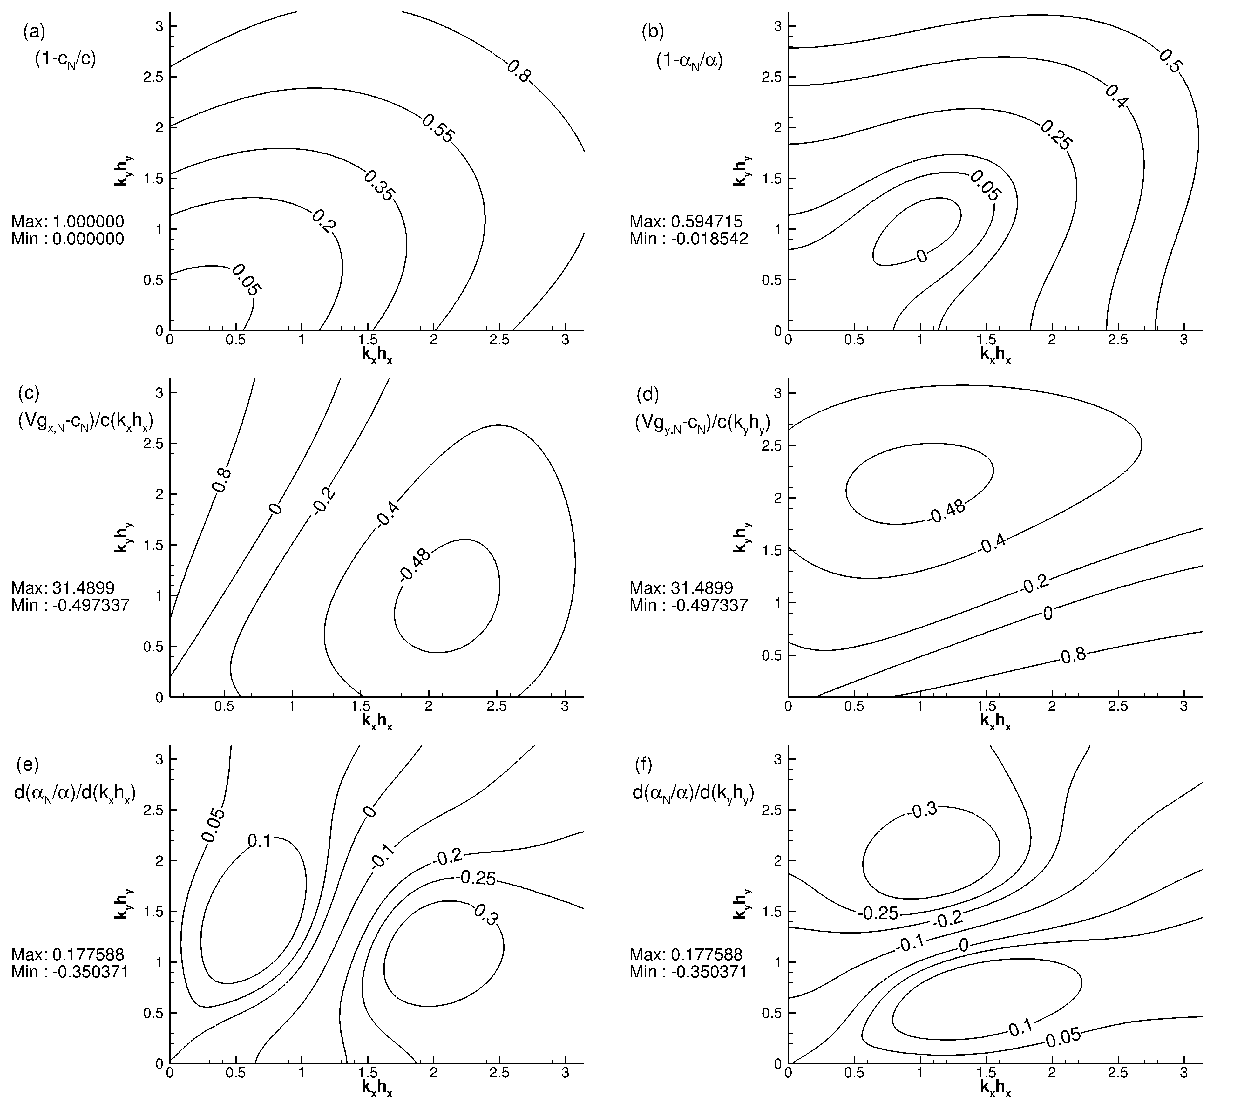
\includegraphics[width=\textwidth]{err_mat_cd2_cd2.pdf}
\end{center}    
\raggedleft
\caption{Contours of error matrices $\left[1-\frac{c_N}{c} \right]$, $\left[1-\frac{\alpha_N}{\alpha}\right]$,$\left[\frac{Vg_{x,N}-c_N}{c(k_xh_x)} \right]$, $\left[\frac{Vg_{y,N}-c_N}{c(k_yh_y)} \right]$, $\left[ \frac{d(\alpha_N/\alpha)}{d(k_xh_x)}\right]$ and $\left[ \frac{d(\alpha_N/\alpha)}{d(k_yh_y)}\right]$ for RK$_4$-CD$_2$-CD$_2$ scheme for $Nc=0.5$ and $Pe=0.01$}
\label{fig_wave}
\end{figure}

For two-dimensional problems, the error propagation equation can be easily formulated by following similar steps as earlier, that can be written in the error matrix form as;
\begin{equation}
\begin{aligned}
\frac{\partial e}{\partial t}+c_x\frac{\partial e}{\partial x}+c_y\frac{\partial e}{\partial y}-\alpha\left(\frac{\partial^2 e}{\partial x^2}+ \frac{\partial^2 e}{\partial y^2}\right) = \alpha &\left[ 1-\frac{\alpha_N}{\alpha}\right] \left(\frac{\partial^2 u_N}{\partial x^2} + \frac{\partial^2 u_N}{\partial y^2}\right) & - c \left[\frac{c_x}{c}-\frac{c_N}{c} \right]\frac{\partial u_N}{\partial x} \\- c \int \left[ \frac{Vg_{x,N}-c_N}{c(k_xh_x)} \right] \left( \frac{\partial u_N}{\partial x} \right) d(k_xh_x)+\alpha \int &\left[ \frac{d(\alpha_N/\alpha)}{d(k_xh_x)}\right] \left( \frac{\partial^2 u_N}{\partial x^2} \right) d(k_xh_x) & - c \left[\frac{c_y}{c}-\frac{c_N}{c}\right]\frac{\partial u_N}{\partial y} \\ - c \int \left[\frac{Vg_{y,N}-c_N}{c(k_yh_y)} \right] \left( \frac{\partial u_N}{\partial y} \right) d(k_yh_y)+ \alpha \int & \left[ \frac{d(\alpha_N/\alpha)}{d(k_yh_y)}\right] \left( \frac{\partial^2 u_N}{\partial y^2} \right) d(k_yh_y)
\end{aligned}
\end{equation}

where all the symbols have their usual meaning as described previously, note that the right-hand side of Eqn. (69) has seven error matrix terms written inside square brackets. First-term represent numerical diffusion error, second and fifth terms represent numerical phase error, and the other four terms represent numerical dispersion error in which third and sixth terms are dispersion due to numerical phase. The fourth and seventh terms are dispersion due to numerical diffusion. If we take $c_x=c_y=c$ ($\textit{i.e.}$ propagation angle, $\theta=45^0$) then the number of error matrix reduces to six.

For any numerical scheme, these six error matrices can be easily calculated using formulation derived from GSA, as explained in the previous section. As an example for two-dimensional case all six error matrices for $RK_4-CD_2-CD_2$ scheme is shown in Fig. \ref{fig_wave} using numerical parameters $Nc=0.5$ and $Pe=0.01$. Distinct contour levels in two-dimensional wavenumber plane $\textit{i.e.}$ ($k_xh_x, k_yh_y$) shown for all six errors matrices with their maximum and minimum values written with them in Fig. \ref{fig_wave}(a) to (f).

\section{Focusing Phenomenon and its Treatment}

The phenomenon of focussing is associated with an abrupt blow-up of a numerical solution after the simulation has gone on for very long computing time. Numerical simulation using multi-level time integration methods are known to blow up abruptly after a long time despite producing entirely accurate results during the time of the simulation. This section explains, \textit{focusing} on the solution of the convection-diffusion equation. It has shown that the obtained properties for the model equation (\textit{i.e.} 2D-CDE) directly apply to the numerical solution of the Navier-Stokes equation \cite{SVajjala2020}. Here, RK$_4$-NCCD scheme has been chosen for the demonstration of the focussing phenomenon, as this numerical scheme shows the best error properties, among others.

\subsection{Effect of $Pe$ on focusing}

Using GSA for the RK$_4$-NCCD scheme, presented in the previous section, the stable and unstable regions in the parameter space can be determined by evaluating whether $|G_N|$ is greater than one or not. In Fig. \ref{fig_NCCD_focus}, we have plotted the curve of $|G_N|$, corresponding to unit value, i.e., $|G_N|=1$ in the wavenumber-axis, for $Nc=0.2$ and $Pe=0.1450671$. The critical value to $Pe$ can be evaluated by plotting iso-surfaces corresponding to $|G_N|=1$ in the three dimensional ($kxhx$, $kyhy$, $Pe$)-plane where iso-surface osculates $Pe$-plane, as given in chapter 1 in \cite{pirozzoli2019}. For higher values of $Pe$, instability is noted at higher ranges of $k_xh_x$ and $k_yh_y$, close to the Nyquist limit. The value of $Pe_{cr}$ decreases when the values of $Nc$ increases beyond a certain limit. By plotting curves in ($Nc, Pe$)-plane for different wave propagation angle, it has observed that $\theta=45^0$ is the most critical case \cite{pirozzoli2019}. The analysis also reveals that instability occurs for a choice of Peclet number $Pe\geq0.1451$ even when $Nc_x=Nc_y=0$.

From the analysis, the first case with $Pe=0.1451$ shows \textit{anti-diffusion}, \textit{i.e.}, $\alpha_N<0$, for the 2D CDE, as noted from the numerical properties shown in Fig. \ref{fig_NCCD_focus}.  One expect the errors to focus in a small region close to the high wavenumbers in the spectral plane, where there is anti-diffusion or $|G_N| > 1$, with grid-scale oscillations. For the other case with $Pe=0.1450671$, the plotted properties for the 2D CDE in Fig. \ref{fig_NCCD_focus} do not show \textit{anti-diffusion} and hence, focusing would be absent for this case.

\begin{figure}[h]
\begin{center}
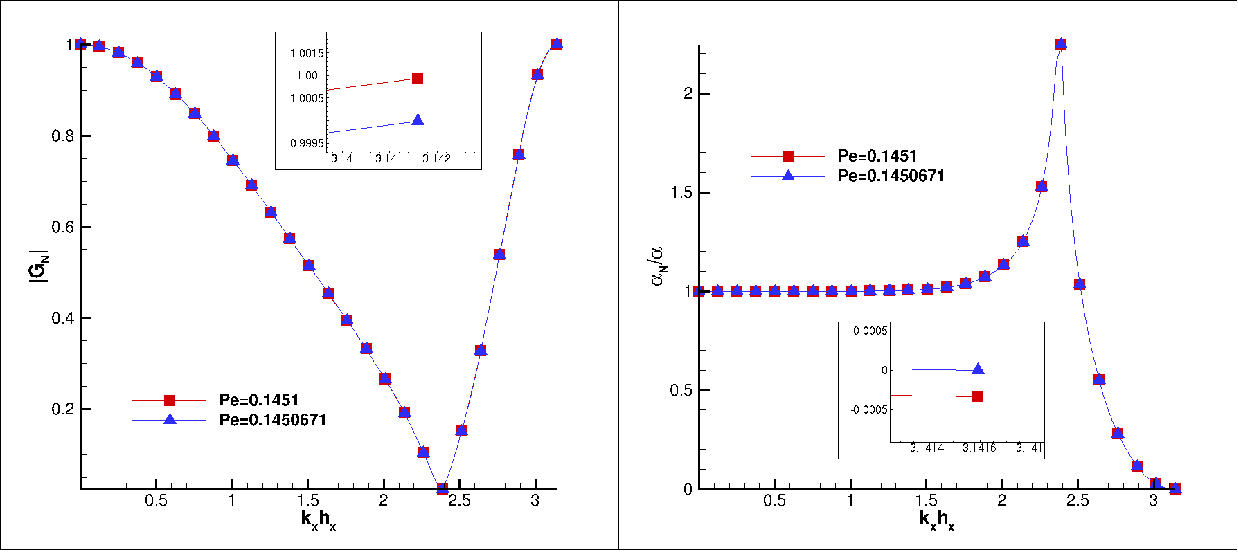
\includegraphics[width=150mm]{NCCD_focus.pdf}
\end{center}
\raggedleft
\caption{Numerical properties of the RK$_4$-NCCD scheme for $Pe=0.1451$ and $Pe=0.1450671$ with same $Nc=0.2$.}
\label{fig_NCCD_focus}
\end{figure}

The observations coming from the analysis has a significant impact on simulations of the unsteady dynamics of the system involving both convection and diffusion processes, particularly for confined geometries. For such problems, a choice of $Pe$ greater than the critical value would lead to a blow-up of solutions within a finite time. This is due to the fact that the solution does not have the means to convect the instabilities out of the computational domain, as is possible for an open flow system. For closed systems, the errors build-up within the domain, continuously affecting the numerical solution, destabilizing the flow due to \textit{anti-diffusion}. This growth of computed solution imitates absolute instability, as has been postulated in \cite{Cossu_et_al}.  In such a case of steady-state simulations, it is interesting to note that one would obtain perfect steady solutions at early times, with the solution matching perfectly with the non-focused solution, but the solution will blow-up after a very long time of simulations. We term such abrupt, but very delayed blow-up in an unsteady manner is due to focussing by the instability in the domain. This phenomenon has been demonstrated in \cite{pirozzoli2019} through the numerical solution of the incompressible Navier-Stokes equation. Where authors performed two simulations for flow inside a 2D square lid-driven cavity problem for same Reynolds number $Re=1000$ and identical $257\ \textsc{x}\ 257$ uniform grid but a slight difference in Peclet number-$Pe$, to demonstrate focusing phenomenon.

\subsection{Effect of non-periodic boundary on focusing}

The boundary closers for a non-periodic boundary problem can also lead to similar problems of focusing. Even if a numerical scheme for a particular value of $Pe$ and $Nc$ produce reasonably good results in terms of properties of GSA \textit{i.e.} $|G_N|$, $|G_N|/|G_{phy}|$, $\alpha_N/\alpha$ and $Vg_N/Vg_x$ values close to unity, boundary closers can some times profoundly affect the overall accuracy of the numerical solution. One such example is shown in Fig. \ref{fig_NCCD_nodes}, where properties of node-2 display distinct features than other nodes in the domain as a consequence of the choice of boundary closer for that node. Its undesirable effects inevitably percolate inside the domain and lead to the tragic situation of blowing up the whole solution for long computing time. In Fig. \ref{fig_NCCD_nodes}, $\alpha_N/\alpha$ values of node-2 after wavenumber $kh=1.0$ reaches its negative value, and hence the value of $|G_N|$ crosses well beyond $1.0$ for high wavenumbers, which is undoubtedly an unstable region.

Hence the study of Global Spectral Analysis is a substantial method in finding out properties of a numerical scheme at every node inside a computational domain by calculating not only its accuracy but also its stability, especially beneficial in very long computational simulations. After the identification of such unstable nodes in the domain, we can implement filtering \cite{sengupta2013high} at that particular node to stabilize the overall solution, a detailed discussion of such a method is in \cite{SENGUPTA_et_al_10}.

\section{Results and Discussion}

\begin{figure}[h]
\begin{center}
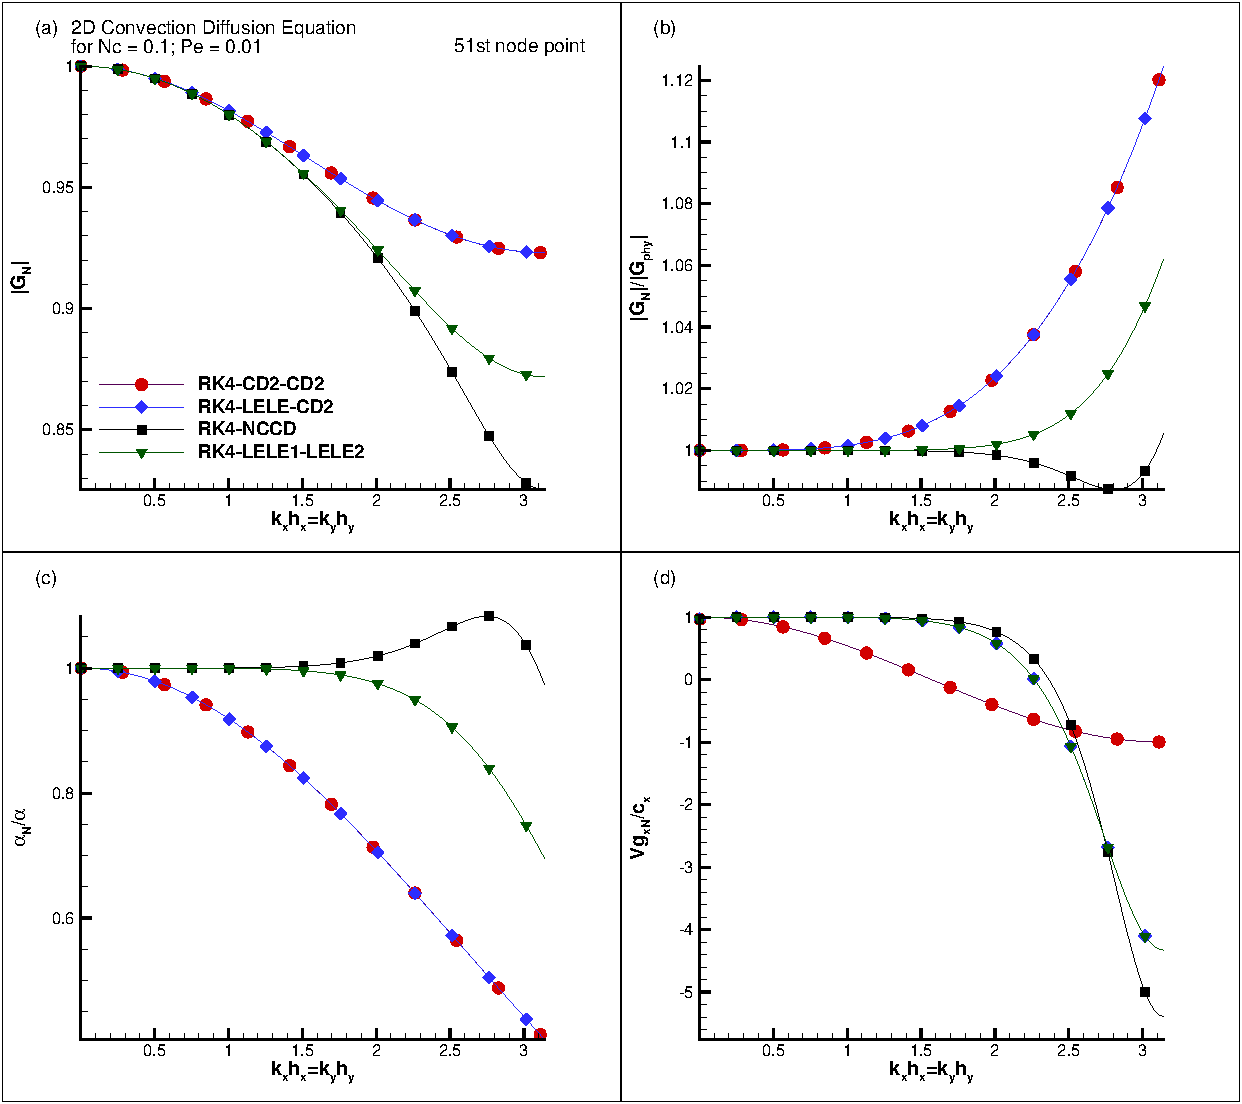
\includegraphics[width=150mm]{all_schemes.pdf}
\end{center}    
\raggedleft
\caption{Plots of $|G_N|$ (top left), $|G_N|/|G_{phy}|$ (top right), $\alpha_N/\alpha$ (bottom left), $Vg_{xN}/Vg_x$ (bottom right) for different schemes, indicated in top left figure, for $Nc=0.1$ and $Pe=0.01$.}
\label{fig_all}
\end{figure}

The global spectral analysis is performed for the 2D linear convection-diffusion equation with the primary objective to explain and demonstrate the accuracy of different numerical schemes with their error matrices. Properties of GSA for various schemes plotted in Fig. \ref{fig_all}, to substantially differentiate their accuracy and stability for a small value of $Nc$ and $Pe$. Better scheme among presented can be specified here by interpreting this figure; hence we conjecture RK$_4$-Lele-Lele$^2$ and RK$_4$-NCCD schemes to be superior to others and the same has been validated below by using them to solve 2D CDE for wave-packet propagation.

\begin{figure}[h]
\begin{center}
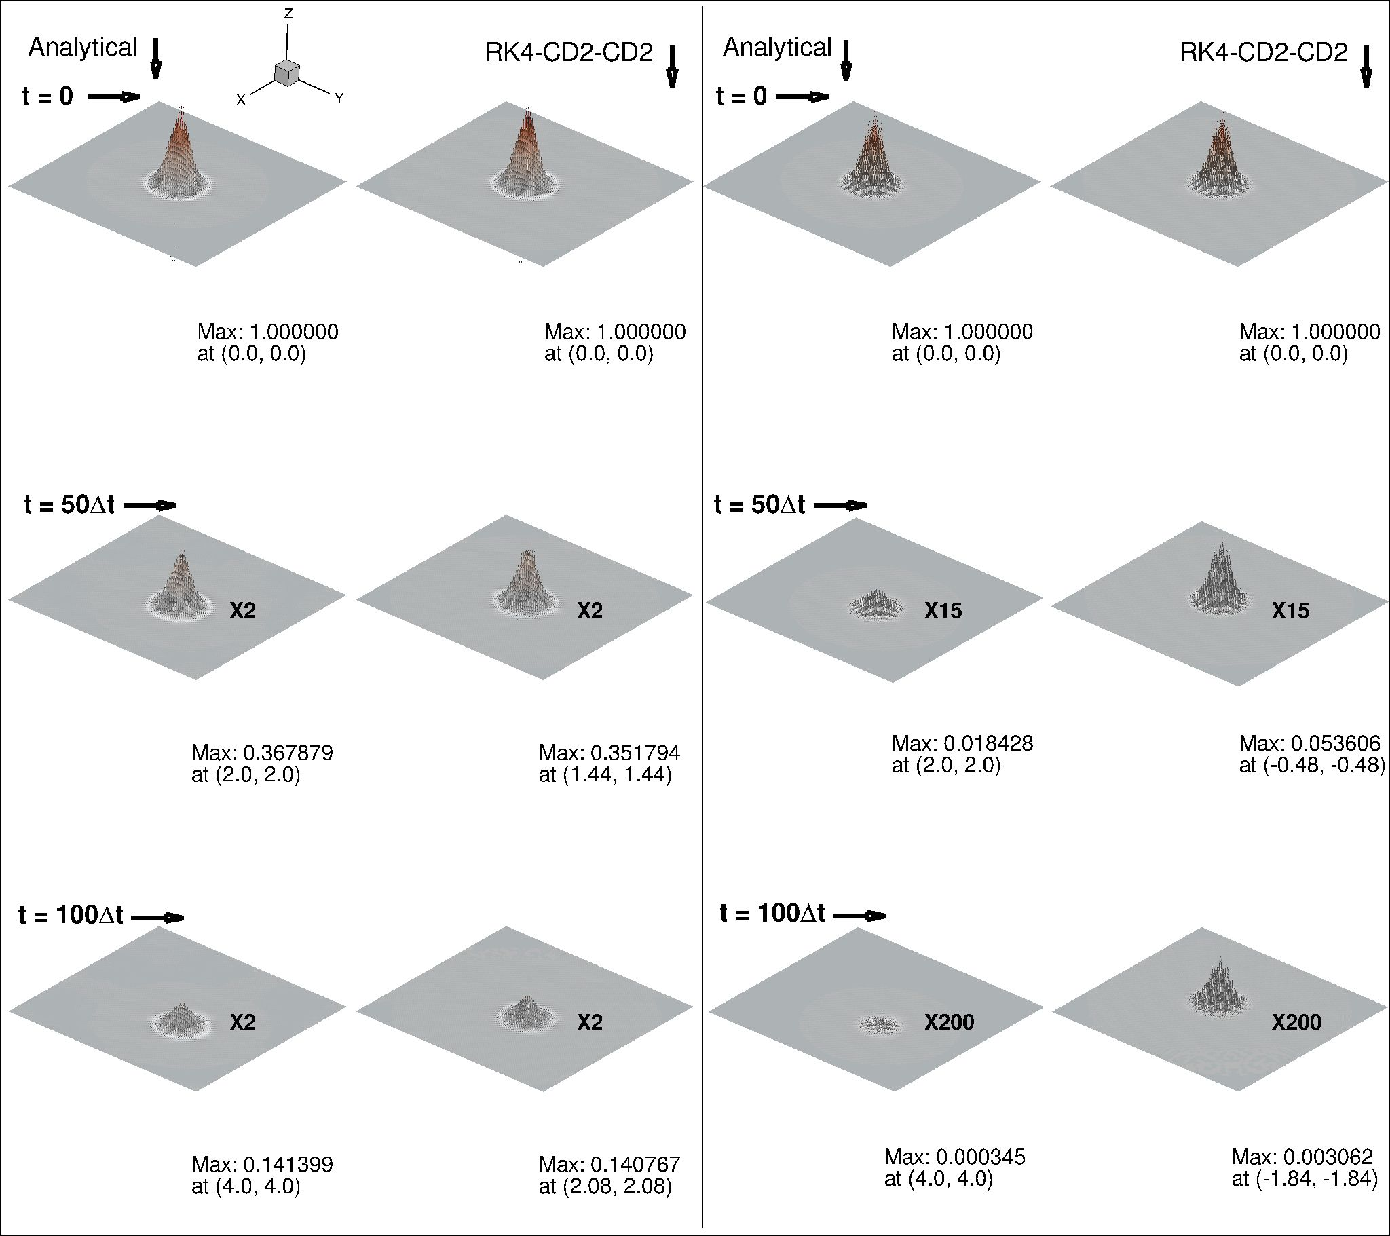
\includegraphics[width=150mm]{wave_pac_cd2_cd2.pdf}
\end{center}    
\raggedleft
\caption{Comparison of 2D wave-packet time evolution; analytical solution (first and third column) with numerical solution (second and fourth column) for wave numbers $k_xh_x=k_yh_y=1.0$ (first two columns) and $k_xh_x=k_yh_y=2.0$ (last two columns) by ensuring $Nc=0.5$ and $Pe=0.01$.}
\label{fig_wave1}
\end{figure}

\begin{figure}[h]
\begin{center}
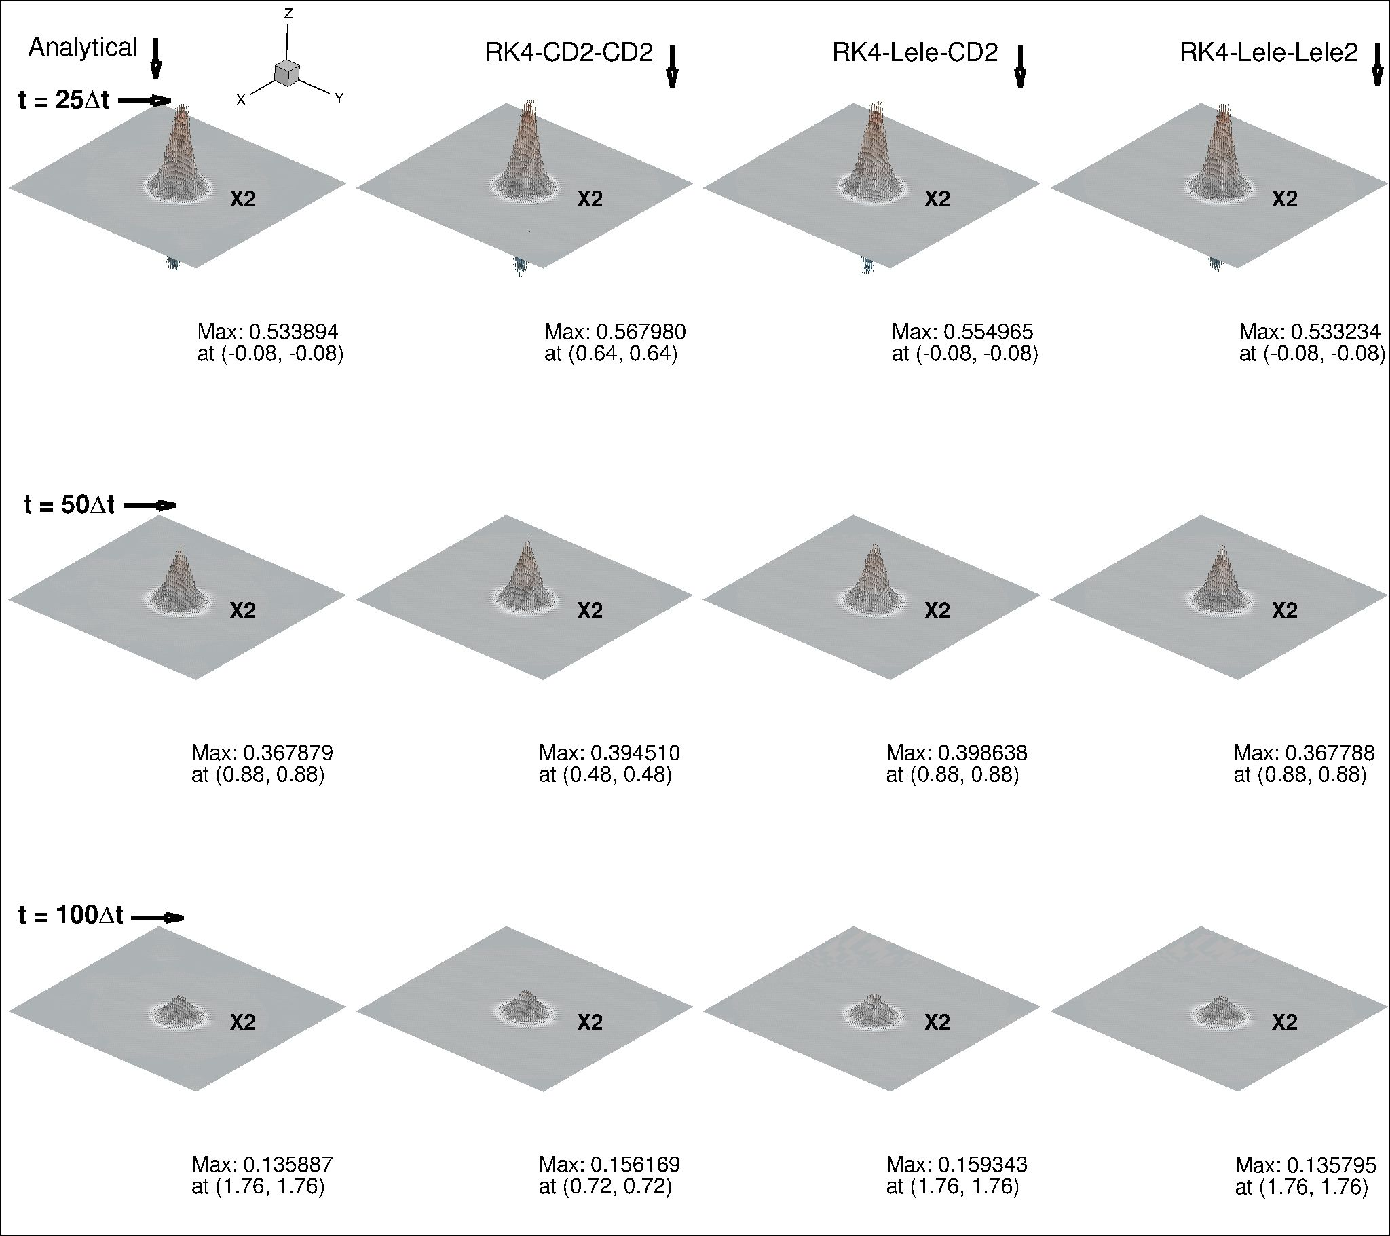
\includegraphics[width=150mm]{wave_pack_all_k1.pdf}
\end{center}    
\raggedleft
\caption{Comparison of 2D wave-packet time evolution; analytical solution (first column) with numerical solution using RK$_4$-CD$_2$-CD$_2$ (second column), RK$_4$-Lele-CD$_2$ (third column) and RK$_4$-Lele-Lele$^2$ (fourth column) for wave numbers $k_xh_x=k_yh_y=1.0$ by ensuring $Nc=0.5$ and $Pe=0.01$.}
\label{fig_wave2}
\end{figure}

The implication of these properties and error matrices in error propagation equation can be noticed by their application in numerically solving 2D CDE by taking 2D wave-packet as an initial state given by,
\begin{equation}
u(x,y,t=0)=e^{-0.16\{(x-x_0)^2+(y-y_0)^2\}} \cos(k_xx).\cos(k_yy) \nonumber
\end{equation}
is considered in the domain of size 40$\times$40 where $x$- and $y$-axis ranges from -20 to 20. We have chosen ($x_0=0$, $y_0=0$) as an initial condition $\textit{i.e.}$ maximum value of wave-packet centered at the origin of coordinates. For the solution of propagation of 2D wave-packet at an angle $\theta=45^0$ we solve 2D CDE, first using RK$_4$-CD$_2$-CD$_2$ numerical scheme for two different set of wave number components, $k_xh_x=k_yh_y=1.0$ and $k_xh_x=k_yh_y=2.0$. We considered the time step $\Delta t=8 \times 10^{-3}$ for all wave-packet simulations, as it attribute to very good numerical accuracy for chosen $Nc$ and $Pe$ values. Fig. \ref{fig_wave1} shows the propagation of wave-packet by solving CDE analytically and numerically in first and second columns in the figure, respectively, for $k_xh_x=k_yh_y=1.0$ at three different time intervals shown in different rows $\textit{i.e.}$ $t=0$, $t=50 \Delta t$, $t=100 \Delta t$. Third and fourth columns in Fig. \ref{fig_wave1} shows analytical and numerical solution of wave-packet for $k_xh_x=k_yh_y=2.0$. The analytical solution is obtained using an analytic technique, in which the initial solution first converted into spectral space using FFT and is advanced at any later time $t$ using Eqn. (11) and resulting solution is converted back into the physical space using the inverse Fourier transform.

The error matrices for chosen $Nc$ and $Pe$ plotted in 2D wave numbers $]\textit{i.e.}$ ($k_xh_x,k_yh_y$)-plane can be seen in Fig. \ref{fig_wave}, and consequently, the behavior of the numerical solution of the wave-packet can be observed by comparing numerical solutions with its analytical counterpart in Fig. \ref{fig_wave1}. By tracing the location of coordinates of the maximum value of wave-packet as labeled in the figures, one can determine the numerical phase and diffusion errors and rate of change of these error quantities $\textit{i.e.}$ numerical dispersion errors in both $x$- and $y$-directions. Note one distinct feature in the simulation that the diffusion matrix ($1-\alpha_N/\alpha$) in the wavenumber plane in Fig. \ref{fig_wave} near $k_xh_x=k_yh_y=1.0$ has a negative value and, therefore, its effect in the numerical solution in Fig. \ref{fig_wave1} can be observed that the maximum amplitude of the wave-packet is smaller in comparison to its value in analytical solution at any time instant, which is in contrast to the other cases. Numbers labeled in figure near the base of wave-packet represents a multiplier of function value $u(x,y,t)$ so that even a very small magnitude of wave-packet can be observed visually.

\begin{table}[h!]
\begin{center}
\caption{Error matrices for $Nc=0.22$ and $Pe=0.01$ at $k_xh_x=k_yh_y=1.0$.}
\label{tab:table1}
\begin{tabular}{|c|c|c|c|c|c|c|c|} % <-- Alignments: columns with vertical lines in between
      \hline
      $S. No.$ & $Scheme(s)$ & $\left(1-\frac{c_N}{c}\right)$ & $\left(1-\frac{\alpha_N}{\alpha}\right)$ & $\left(\frac{Vg_{xN}-c_N}{c(k_xh_x)}\right)$ & $\left(\frac{Vg_{yN}-c_N}{c(k_yh_y)}\right)$ & $\left(\frac{d(\alpha_N/\alpha}{d(k_xh_x)}\right)$ & $\left(\frac{d(\alpha_N/\alpha}{d(k_yh_y)}\right)$ \\
      \hline
      1 & $RK_4-CD_2-CD_2$ & 0.15869 & 0.08045 & -0.3015 & -0.3015 & -0.0779 & -0.0779\\
      2 & $RK_4-Lele-CD_2$ & 0.00085 & 0.07953 & -0.0046 & -0.0046 & -0.0756 & -0.0756\\
      3 & $RK_4-Lele-Lele_2$ & 0.00085 & -0.00064 & -0.00464 & -0.00464 & 0.00096 & 0.00096\\
      \hline
\end{tabular}
\end{center}
\end{table}

\begin{figure}[h]
\begin{center}
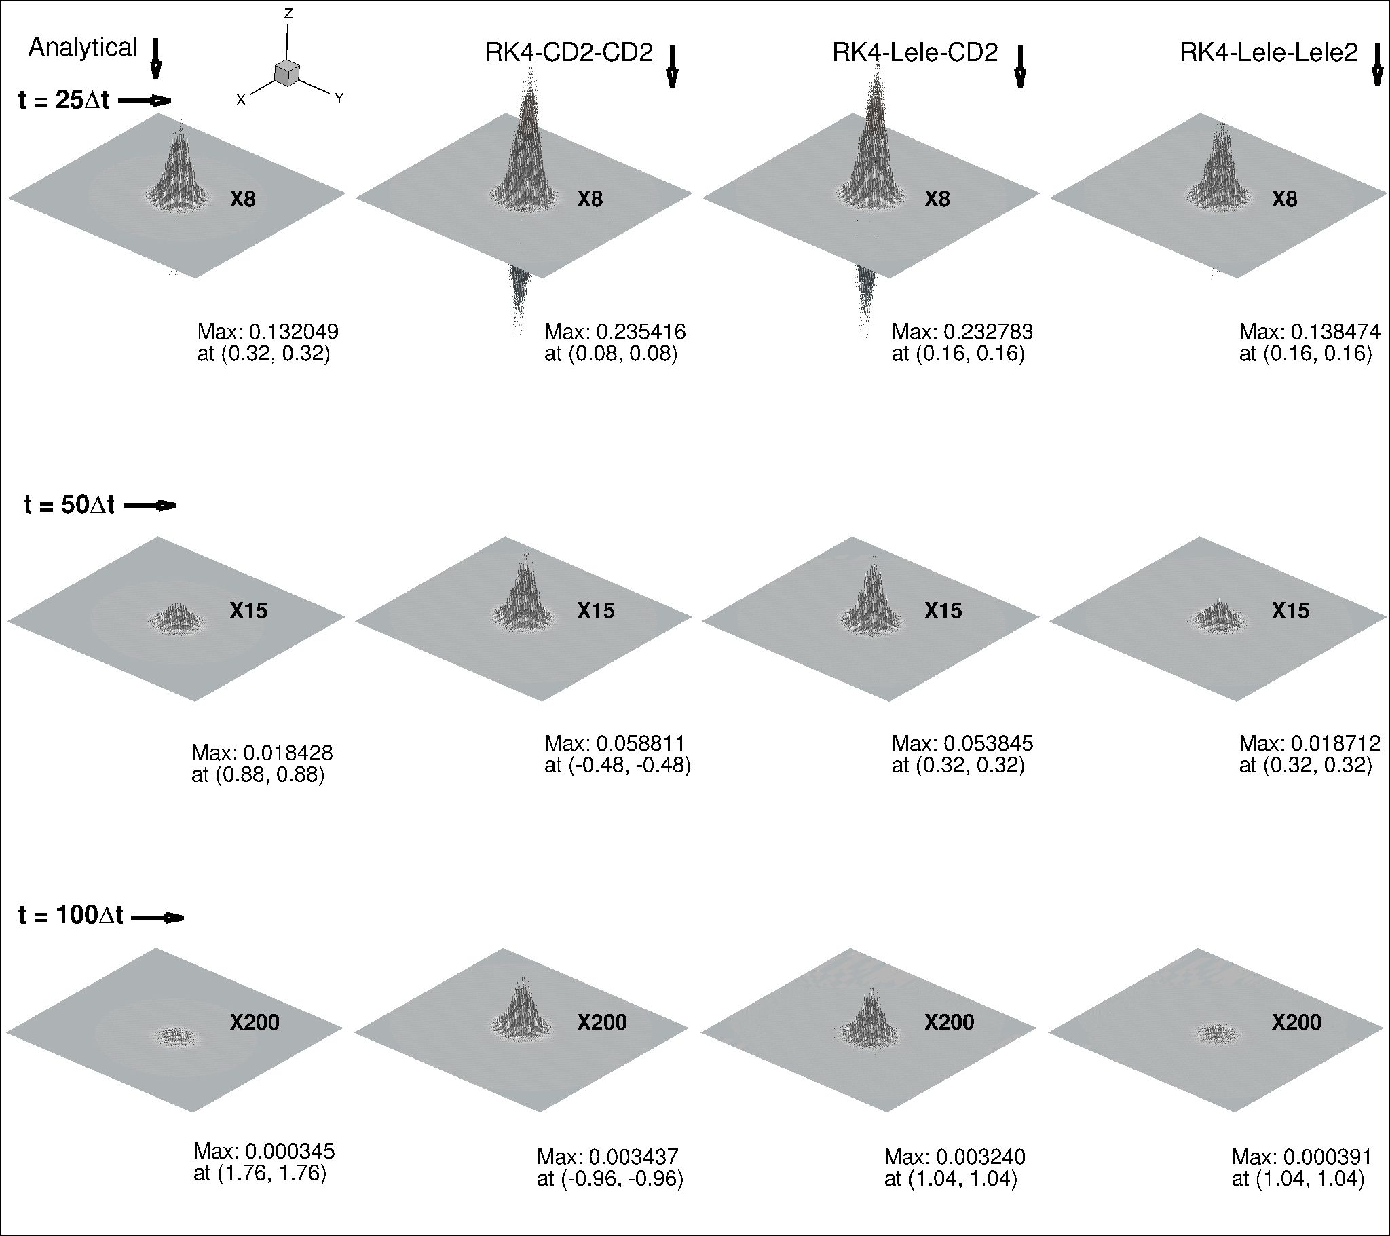
\includegraphics[width=150mm]{wave_pack_all_k2.pdf}
\end{center}    
\raggedleft
\caption{Comparison of 2D wave-packet time evolution; analytical solution (first column) with numerical solution using RK$_4$-CD$_2$-CD$_2$ (second column), RK$_4$-Lele-CD$_2$ (third column) and RK$_4$-Lele-Lele$^2$ (fourth column) for wave numbers $k_xh_x=k_yh_y=2.0$ by ensuring $Nc=0.5$ and $Pe=0.01$.}
\label{fig_wave}
\end{figure}

Now we calculate error matrices using three different numerical schemes to make a comparison of accuracy between the numerical schemes using error propagation equation. For a combination of $Nc=0.22$ and $Pe=0.01$, error matrices have been calculated using the same technique as above, for two different values of wavenumbers. Six error matrices for RK$_4$-CD$_2$-CD$_2$, RK$_4$-Lele-CD$_2$ and RK$_4$-Lele-Lele$_2$ numerical schemes has been shown in Table I and Table II for wave numbers $k_xh_x=k_yh_y=1.0$ and $k_xh_x=k_yh_y=2.0$, respectively. Fig. \ref{fig_wave2} represents analytical and numerical results of 2D CDE using above mentioned numerical schemes for $k_xh_x=k_yh_y=1.0$. In this figure time evolution of a wave-packet exhibit solution at three different intervals without showing initial condition, as it is same as shown in Fig. \ref{fig_wave1}.

\begin{table}[h!]
  \begin{center}
    \caption{Error matrices for $Nc=0.22$ and $Pe=0.01$ at $k_xh_x=k_yh_y=2.0$.}
    \label{tab:table2}
    \begin{tabular}{|c|c|c|c|c|c|c|c|} % <-- Alignments: 1st column left, 2nd middle and 3rd right, with vertical lines in between
      \hline
      $S. No.$ & $Scheme(s)$ & $\left(1-\frac{c_N}{c}\right)$ & $\left(1-\frac{\alpha_N}{\alpha}\right)$ & $\left(\frac{Vg_{xN}-c_N}{c(k_xh_x)}\right)$ & $\left(\frac{Vg_{yN}-c_N}{c(k_yh_y)}\right)$ & $\left(\frac{d(\alpha_N/\alpha}{d(k_xh_x)}\right)$ & $\left(\frac{d(\alpha_N/\alpha}{d(k_yh_y)}\right)$ \\
      \hline
      1 & $RK_4-CD_2-CD_2$ & 0.54547 & 0.2924 & -0.4350 & -0.4350 & -0.1265 & -0.1265\\
      2 & $RK_4-Lele-CD_2$ & 0.05419 & 0.276297 & -0.18089 & -0.18089 & -0.11975 & -0.11975\\
      3 & $RK_4-Lele-Lele_2$ & 0.05446 & 0.01293 & -0.18159 & -0.18159 & -0.03439 & -0.03439\\
      \hline
    \end{tabular}
  \end{center}
\end{table}

Numerical schemes $RK_4-CD_2-CD_2$ and $RK_4-Lele-CD_2$ has approximately same values of ($1-\alpha_N/\alpha$) for $k_xh_x=k_yh_y=1.0$ as shown in Table I, therefore the effect of numerical diffusion is same in the simulation of wave-packet plotted in Fig. \ref{fig_wave2}, where the maximum amplitude is nearly the same, but the later scheme displays a significant improvement in the convection of wave-packet $\textit{i.e.}$ location of maximum amplitude is closer to the analytical value, the reason for this is rectification in its ($1-c_N/c$) value. $RK_4-Lele-Lele_2$ scheme exhibits the best error control, as indicated by Table I; hence it leads to the best simulation results for CDE. Similar results can be seen in Fig. \ref{fig_wave3}, simulation of wave-packet for $k_xh_x=k_yh_y=2.0$ with less accuracy than Fig. \ref{fig_wave2} due to the notable increment in error matrices corroborated clearly in Table II.

\section{Conclusion and Summary}

A global spectral analysis of numerical schemes based on the finite difference method for the 2D linear convection-diffusion equation presented in this current study. Exact properties of this equation, as well as numerical amplification factor and critical parameters, such as $\frac{|G_N|}{G}$, $\frac{\alpha_N}{\alpha}$, $\frac{c_N}{c}$ and $\frac{V_{g,N}}{c}$ derived in order to measure the accuracy and stability of numerical schemes. The analysis suggests that numerical schemes gain accuracy when these properties reach close to unity for the entire wavenumber range. The second aim of this study is to investigate the correct error propagation equation for the convection-diffusion equation that accounts for the numerical phase, diffusion, and dispersion errors. This analysis shows that the change in physical phase speed and physical diffusion constant to the variable numerical phase speed $c_N$ and numerical diffusion constant $\alpha_N$, a function of wavenumber, which leads to additional forcing terms on the right-hand side of Eqn. (69) dependent upon the errors, and the spatial gradients of the numerical solution.

RK$_4$-CD$_2$-CD$_2$, RK$_4$-Lele-CD$_2$ and RK$_4$-Lele-Lele$^2$ schemes are analyzed in this work and numerical tests performed for 2D wave-packet propagation for which exact solution is available for comparison. Among these schemes, RK$_4$-Lele-Lele$^2$ scheme showed the best accuracy for specific $Nc$ and $Pe$ values. Numerical computations demonstrate lower diffusion and convection errors for all time intervals of a 2D wave-packet propagation using the scheme above. This research on the linear convection-diffusion equation suggests that before proceeding to solve any such problems using finite-difference methods, such a study should carry out first. So that careful choice of numerical parameters can be made for the better accuracy and stability of numerical schemes by the study of boundary closers for the chosen grid or the total number of nodes in the computational domain.

\clearpage
\bibliography{ank_b.bib}
%\bibliography{pks.bib}
%\clearpage
%\input{ank_figures.tex}

%%%%%%%%%%%%%%%%%%%%%%%%%%%%%%%%%%%%%%%%%%%%%%%%%%%%%%%%%%%%%%

\end{document}
